\documentclass{Template/thesisclass}
\usepackage[utf8]{inputenc}

\author{Christian Schnorr}
\title{Visualizing dynamic clustered data using area-proportional maps}
\date{November 14th, 2019 \@ -- \@ May 13th, 2020}

\makeatletter
\hypersetup{
	pdfauthor={\@author},
	pdftitle={\@title},
}
\makeatother

\usepackage{amsmath}
\usepackage{amssymb}
\usepackage{mathtools}

\newcommand{\clustergraph}[1]{\ensuremath{G^\mathcal{C}_{#1}}}
\newcommand{\initmap}[1]{\ensuremath{\Gamma^*_{#1}}}
\newcommand{\propmap}[1]{\ensuremath{\Gamma^\propto_{#1}}}
\DeclareMathOperator{\Perp}{Perp}
\DeclareMathOperator{\Bsc}{Bisect}
\DeclareMathOperator{\Norm}{Norm}

% Functions

\newcommand{\eval}[2]{{#1}{\left({#2}\right)}}
\newcommand{\floor}[1]{\left\lfloor#1\right\rfloor}
\newcommand{\ceil}[1]{\left\lceil#1\right\rceil}


% Algebra

\newcommand{\abs}[1]{\left\lvert#1\right\rvert}
\newcommand{\norm}[1]{\left\lVert#1\right\rVert}


% Calculus

\newcommand{\differential}[1]{\mathop{d #1}}


% Geometry

\newcommand{\segment}[1]{\overline{#1}}
\newcommand{\longvec}[1]{\overrightarrow{#1}}
\newcommand{\degrees}{^{\circ}}


% Big O notation

\newcommand{\bigOh}[1]{\mathcal{O}(#1)}
\newcommand{\bigTheta}[1]{\Theta(#1)}
\newcommand{\bigOmega}[1]{\Omega(#1)}


% Graph Theory

\newcommand{\indeg}{deg^{-}}
\newcommand{\outdeg}{deg^{+}}


% Set Theory

\newcommand{\cupplus}{\uplus}

\usepackage{amsthm}
\usepackage{float}
\usepackage[inline]{enumitem}

\theoremstyle{definition}
\newtheorem{definition}{Definition}[chapter]

\theoremstyle{definition}
\newtheorem{theorem}{Theorem}[chapter]

\theoremstyle{definition}
\newtheorem{lemma}{Lemma}[chapter]

\theoremstyle{definition}
\newtheorem{proposition}{Proposition}[chapter]

\theoremstyle{definition}
\newtheorem{corollary}{Corollary}[chapter]

\theoremstyle{definition}
\let\oldproofname=\proofname
\renewcommand{\proofname}{\rm\bf{\oldproofname}}

\theoremstyle{remark}
\newtheorem*{remark}{Remark}

\theoremstyle{plain}

\SetKwInput{KwData}{Input}
\SetKwInput{KwResult}{Output}
\DontPrintSemicolon

\newcommand{\code}{\texttt}

\usepackage{hyperref}
\usepackage{cite}
\usepackage{doi}

\usepackage{cleveref}

\crefname{chapter}{Chapter}{Chapters}
\Crefname{chapter}{Chapter}{Chapters}
\crefname{section}{Section}{Sections}
\Crefname{section}{Section}{Sections}
\crefname{equation}{Equation}{Equations}
\Crefname{equation}{Equation}{Equations}
\crefname{figure}{Figure}{Figures}
\Crefname{figure}{Figure}{Figures}
\crefname{theorem}{Theorem}{Theorems}
\Crefname{theorem}{Theorem}{Theorems}
\crefname{lemma}{Lemma}{Lemmata}
\Crefname{lemma}{Lemma}{Lemmata}
\crefname{line}{line}{lines}
\Crefname{line}{Line}{Lines}
\crefname{algorithm}{Algorithm}{Algorithms}
\Crefname{algorithm}{Algorithm}{Algorithms}

\numberwithin{equation}{chapter}
\numberwithin{figure}{chapter}
\numberwithin{algocf}{chapter}

\newcommand{\hiddensubsection}[1]{\stepcounter{subsection}\subsection*{\arabic{chapter}.\arabic{section}.\arabic{subsection}\hspace{1.25ex}{#1}}}

\newcommand{\ie}[0]{i.\,e.\@}
\newcommand{\eg}[0]{e.\,g.\@}
\newcommand{\etal}[0]{et al.\@}

\newcommand{\emdash}{---}

\newcommand{\lipsum}{Lorem ipsum dolor sit amet, consectetur adipiscing elit. Sed a elementum nibh. Sed elementum odio nec erat commodo sollicitudin. Vivamus dolor arcu, ultrices ut condimentum sit amet, fermentum id ante. Vestibulum suscipit ut ex efficitur pellentesque. Maecenas non mollis enim. Nullam commodo purus vel fringilla lobortis. Lorem ipsum dolor sit amet, consectetur adipiscing elit. Etiam fringilla commodo tellus, quis semper lacus fermentum sed. Mauris id rhoncus neque, eu elementum ligula. Interdum et malesuada fames ac ante ipsum primis in faucibus. Nam ac ligula eleifend, pulvinar libero ac, lacinia quam. Integer aliquam eget nunc ac finibus. Phasellus nisl ante, ornare sit amet accumsan vitae, scelerisque ut nulla. Suspendisse potenti. Suspendisse ac placerat ipsum. Proin eget ligula velit.}

\newcommand{\todo}[1]{\textcolor{red}{TODO: #1}}
\newcommand{\quoted}[1]{``#1''}


%\includeonly{Sources/01-Introduction,Sources/02-Preliminaries}
%\includeonly{Sources/02-Preliminaries,Sources/03-Visualizing-Static-Input-Graphs}
%\includeonly{Sources/02-Preliminaries,Sources/08-Bibliography}
%\includeonly{Sources/01-Introduction,Sources/02-Preliminaries,Sources/03-Visualizing-Static-Input-Graphs,Sources/04-Visualizing-Dynamic-Input-Graphs,Sources/07-Bibliography}
%\includeonly{Sources/03-Visualizing-Static-Input-Graphs,Sources/04-Visualizing-Dynamic-Input-Graphs,Sources/07-Bibliography}
%\includeonly{Sources/02-Preliminaries,Sources/04-Visualizing-Dynamic-Input-Graphs}
%\includeonly{Sources/03-Visualizing-Static-Input-Graphs}
\includeonly{Sources/04-Visualizing-Dynamic-Input-Graphs}
%\raggedbottom

\begin{document}
\selectlanguage{american}
\makeatletter
\hypersetup{
  pdfauthor={\@author},
  pdftitle={\@title},
}
\makeatother

\makeatletter
\begin{titlepage}

\begin{tikzpicture}[overlay]
  \newcommand{\diameter}{7}
  \newcommand{\xone}{-15}
  \newcommand{\xtwo}{160}
  \newcommand{\yone}{15}
  \newcommand{\ytwo}{-253}
  \draw[color=gray]
  (\xone mm, \yone mm)
  -- (\xtwo mm, \yone mm)
  arc (90:0:\diameter mm)
  -- (\xtwo mm + \diameter mm , \ytwo mm)
  -- (\xone mm + \diameter mm , \ytwo mm)
  arc (270:180:\diameter mm)
  -- (\xone mm, \yone mm);
\end{tikzpicture}

\begin{textblock}{10}[0,0](4,2.5)

\includegraphics[width=.3\textwidth]{Resources/Logos/KIT.pdf}
\end{textblock}

\begin{textblock}{10}[0,0](14.5,2.45)

\includegraphics[width=.15\textwidth]{Resources/Logos/Algo.pdf}
\end{textblock}


\changefont{phv}{m}{n}
\vspace*{3.75cm}

\begin{center}
  \Huge{\@title}
  \vspace*{2.25cm}\\
  \Large{Master Thesis of}\\
  \vspace*{1cm}
  \huge{\@author}\\
  \vspace*{1cm}
  \Large{At the Department of Informatics}\\
  \Large{Institute of Theoretical Informatics, Algorithmics I}\\
\end{center}

\vspace*{1cm}

\begin{center}
\begin{Large}
\begin{tabular}[ht]{l c l}
  Reviewer: & \hfill & Prof.~Dr.~Dorothea Wagner\\
  Advisor: & \hfill & Dr.~Tamara Mchedlidze
\end{tabular}
\end{Large}
\end{center}

\vspace{2cm}

\begin{center}
\large{Time Period:~~\@date}
\end{center}

\begin{textblock}{10}[0,0](4,16.8)
\tiny{KIT -- The Research University in the Helmholtz Association}
\end{textblock}

\begin{textblock}{10}[0,0](14,16.75)
\large{\textbf{www.kit.edu}}
\end{textblock}

\end{titlepage}
\makeatother


\blankpage

\thispagestyle{plain}

\centerline{\textbf{Acknowledgements}}
\vspace{0.25cm}

First of all, I would like to thank my advisor, {Dr.~Tamara Mchedlidze}, for making this project possible through our weekly meetings and fruitful discussions, valuable feedback, and pointers in the right direction.

I am also grateful to the Algorithmics Group of {Prof.~Dr.~Dorothea Wagner} for the interesting courses over the last years, for giving me the opportunity to write this thesis, for their valuable insights early on in the project, and for the overall pleasant atmosphere.

Last but by no means least, I would like to thank my parents and grandparents and my good friend Johannes Hubert for their unfailing support and encouragement that kept me motivated on this final stretch, and for lending me some cores to help me crunch numbers for the evaluation of the framework discussed in this thesis.

Thank you!

\vspace*{\fill}



\centerline{\textbf{Statement of Authorship}}
\vspace{0.25cm}

I hereby declare that this document has been composed by myself and describes my own work, unless otherwise acknowledged in the text.

\vspace{2.5cm}

\noindent
\makebox[7.5cm]{\hrulefill}

\hspace{0.25cm}
Karlsruhe, \today

\vspace{2cm}


\blankpage

\thispagestyle{plain}

% https://www.easterbrook.ca/steve/2010/01/how-to-write-a-scientific-abstract-in-six-easy-steps/
% The first sentence of an abstract should clearly introduce the topic of the paper so that readers can relate it to other work they are familiar with.
% However, an analysis of abstracts across a range of fields show that few follow this advice, nor do they take the opportunity to summarize previous work in their second sentence.
% A central issue is the lack of structure in standard advice on abstract writing, so most authors don’t realize the third sentence should point out the deficiencies of this existing research.
% To solve this problem, we describe a technique that structures the entire abstract around a set of six sentences, each of which has a specific role, so that by the end of the first four sentences you have introduced the idea fully.
% This structure then allows you to use the fifth sentence to elaborate a little on the research, explain how it works, and talk about the various ways that you have applied it, for example to teach generations of new graduate students how to write clearly.
% This technique is helpful because it clarifies your thinking and leads to a final sentence that summarizes why your research matters.

\begin{addmargin}{0.5cm}

\centerline{\textbf{Abstract}}

In this thesis, we explore how cluster information in graphs can be visualized naturally as countries on a map in a dynamic setting where the graph changes over time.
We want there to be a strong correlation between a country's size and the size of the cluster it represents, and want to be able to react to dynamic changes of the graph in a way that preserves the viewer's mental model of the map.
This is a challenging problem because popular algorithms for visualizing graphs as geographic-like maps struggle with clusters being fragmented across different countries on the map, and because redrawing the map for a new, albeit similar, input graph does generally not preserve the viewer's mental map.

To address these issues, we propose a framework that guarantees to keep clusters as continuous regions in the generated maps and supports dynamic inputs by allowing for small, incremental updates such as inserting or removing regions over time.
We do this by working on an intermediate plane graph whose vertices correspond to clusters in the input graph, the cluster graph, and constructing the map as a contact representation of this cluster graph while accounting for the dynamic changes in both the cluster graph and its contact representation.
This framework can be applied to a variety of real-world applications, allowing us to visualize clusters in the underlying data and how they change over time, thereby enabling viewers of the visualization to easily detect trends in the data.

\vskip 2cm

\centerline{\textbf{Deutsche Zusammenfassung}}

\selectlanguage{ngerman}
In der vorliegenden Arbeit untersuchen wir, wie Clusterinformationen in Graphen als Länder einer Landkarte dargestellt werden können, wobei sich der Eingabegraph mit der Zeit verändert.
Wichtig ist dabei eine starke Korrelation zwischen der Größe eines Landes auf der Karte und der Größe des entsprechenden Clusters.
Außerdem wollen wir so auf Änderungen des Eingabegraphen reagieren können, dass ein Betrachter seine Orientierung auf der Karte nicht verliert.
Das ist eine herausfordernde Problemstellung, da gängige Algorithmen zur landkartenähnlich Visualisierung von Graphen mit Clustern zu kämpfen haben, die über mehrere Länder auf der Karte fragmentiert sind.
Außerdem geht die Orientierung des Betrachters bei einer Neuzeichnung der Karte für einen anderen, wennauch sehr ähnlichen Graphen, im Allgemeinen verloren.

Zur Lösung dieser Probleme schlagen wir ein Rahmenkonzept vor, welches garantiert, dass die Cluster jeweils zusammenhängende Regionen auf der Karte bilden.
Außerdem werden dynamische Eingaben insofern unterstützt, als dass kleine, inkrementelle Änderungen wie z.B. das Einfügen oder Entfernen einer Region, durchgeführt werden können.
Dafür arbeiten wir auf einem Hilfsgraphen, dessen Knoten den Clustern im Eingabegraph entsprechen, konstruieren die Karte als Kontaktrepräsentation dieses Graphen und passen bei Änderungen am Eingabegraphen sowohl den Hilfsgraphen als auch dessen Kontraktrepräsentation entsprechend an.
Dieser Ansatz kann für eine Vielzahl von Anwendungen benutzt werden, um Cluster und deren zeitliche Enwicklung auf eine natürliche Art und Weise darzustellen und es dem Betrachter somit zu erleichtern, Trends in den zugrundeliegenden Daten zu erkennen.
\selectlanguage{american}

\end{addmargin}


\blankpage

\tableofcontents

\chapter{Introduction}
\label{chap:introduction}

% Visualizing dynamic clustered data using area-proportional maps

\section{Motivation}
\label{sect:motivation}

We live in a world with an abundance of data. Data for which it is no longer possible for humans alone to work through, to make sense of, and data that is only going to increase in volume in the years to come. As the amount of data we work with grows, it becomes increasingly important to properly visualize the data in order to gain key understandings and to communicate those with others. It is crucial to make use of this visual perception channel as it has the highest information bandwidth of all our senses. In fact, humans acquire more information through vision alone than through all other senses combined \cite{ware2019information}.

As the amount of data that needs to be visualized keeps growing while the human ability to process data remains constant, it becomes increasingly important to capture the most relevant aspects of the data \cite{dachsbacher2019visualisierung}. In the field of graph theory and graph drawing, for example, for larger graphs, global structures such as clusters and their relationships become increasingly important while local features such as individual edges loose importance.

\new{
Saket \etal{} \cite{saket2014group} propose a set of tasks that assess a user's ability to detect clustering information in graph visualizations. They evaluated these tasks across different types of diagrams \cite{saket2014node} and found that node-link-group diagrams, \ie{} diagrams in which there is an explicit representation of clusters, outperform both node and node-link diagrams on group-based tasks and do not negatively affect the performance of other tasks. According to another study by Saket \etal{} \cite{saket2016comparing}, node-link-group diagrams are also more enjoyable for users to work with. In this thesis, we make use of the map metaphor and encode the clustering information by placing all vertices of a cluster in the same \quoted{country} of a map.
}

But in today's world it's not only big data that we're dealing with. Data is also changing at a much greater pace than before. Visualizations that were accurate a moment ago may be outdated now. For many applications it is therefore crucial to visualize how data evolves over time \emdash{} maybe even more so than a snapshot of the data at a single point in time.

A core motivating application for this thesis is visualizing an \emph{opinion network} \cite{betz2019applying} and in particular visualizing how it evolves over time: An opinion network is represented as a weighted graph whose vertices are so-called \emph{opinion vectors} and the edge weights represent the similarity between two opinion vectors. Betz \etal{} cluster the vertices to group similar opinions together, visualize the graph as a map in which each cluster corresponds to a country, and draw the original graph on top of this map. Naturally, such an opinion network is dynamic in a sense where new opinions can be incorporated or individual opinions can change over time. Therefore clusters can grow or shrink, appear or disappear, merge or split, and we are interested in visualizing this underlying process over time.

\cite{dobbins2018forall}

\section{Related Work}
\label{sect:related-work}

%three core components/requirements/objectives:
%- area-proportional maps
%- dynamic aspect
%- natural shapes

% skewed, distorted, deformed
% variable of interest, statistic

While a vertex-weighted cluster graph is the intuitive representation of the data we want to visualize, we'll end up doing most of the work in the following chapters on the dual problem: We transform the vertex-weighted cluster graph into its dual graph. The weights then apply to the faces of dual graphs and we are looking to draw the dual such that the faces have some prescribed area. A drawing of the dual essentially is a \emph{contact representation} of the original graph: iff two faces share part of their boundaries, the corresponding vertices in the original graph are adjacent.

\emph{Area-universal graphs} are graphs that can realize any area assignment to its inner faces with straight-line edges. Research on area-universality give us important theoretical bounds on the statistical accuracy we can achieve with polygonal countries: Back in 1992, Thomassen \cite{thomassen1992plane} showed that plane cubic graphs are area-universal. This means that we can achieve perfect statistical accuracy with straight-line edges for the dual of any triangulated graph. Kleist \cite{kleist2018drawing} \cite{kleist2019planar} showed that the 1-subdivision of any plane graph is area-universal. Therefore with just one bend per edge, any plane graph can be drawn with any prescribed face areas. Biedl and Velázquez \cite{biedl2013drawing} showed that the class of 3-trees and subgraphs thereof are area-universal, providing a constructive proof based on barycentric coordinates.

Drawing graphs with prescribed face areas is also closely related to so-called \emph{cartograms}. Cartograms are maps in which geographic regions appear skewed such that their areas are proportional to some statistic, \eg{} the population or gross domestic product of a country. Cartograms have been studied for more than 50 years \cite{tobler2004thirty} and there are many fundamentally different approaches to generate different kinds of cartograms \cite{nusrat2016state}. The effectiveness of cartograms related to human perception has been evaluated extensively \cite{nusrat2018evaluating} and the following three quantitative metrics are most commonly used to judge the quality of cartograms \cite{nusrat2016state} \cite{alam2015quantitative} \cite{nusrat2018evaluating}:
%
\begin{itemize}
	\item \emph{Statistical accuracy}: How closely do the modified geographic areas represent the variable of interest?
	\item \emph{Topological accuracy}: How well is the map topology, \ie{} the adjacency relationship between geographic regions, preserved?
	\item \emph{Geographic accuracy}: How closely do the distorted geographic shapes and positions resemble their original?
\end{itemize}

Although cartograms are traditionally used to visualize demographic data on real geographic maps, they are closely related to the problem at hand: visualizing clusters such that their areas are proportional to their sizes, \ie{} the number of vertices. Statistical and topological accuracy still apply, but geographical accuracy becomes a meaningless quality metric because the visualization isn't based on any natural geographic map and there are no \quoted{original} versions of the country shapes.

Nusrat and Kobourov \cite{nusrat2016state} give an overview of many different algorithms for generating cartograms and discuss how they stack up against one another.

Gastner and Newman \cite{gastner2004diffusion} propose a physical model based on diffusion to generate cartograms: They rasterize the original map into a two-dimensional matrix with the values being the initial densities, \ie{} the statistical values divided by the regions' areas at any given point. This matrix is then used to precompute the gradient of the diffusion field and the pathlines of these \quoted{density particles} as they diffuse through the map and equalize the overall density. The pathlines essentially map locations on the original map to their location in the diffused map and can be used to draw the distorted, density-equalizing map. Due to the rasterization and heavy precomputation of pathlines, this algorithm isn't well-suited for our dynamic setting in which densities can change.

Kämper \etal{} \cite{kamper2013circular} start with a polygonal map and transform every edge into a circular arc that can bend to realize the desired areas of individual regions. They use a max-flow-based formulation on the dual graph of the map to find out how the area should be distributed among the regions and solve for the circular arc radii. However the degree to which the edges can bend is heavily restricted since the circular arcs may not touch or cross, making it difficult for circular arc cartograms to achieve good statistical accuracies.

Alam \etal{} \cite{alam2013computing} show how air-pressure-based models for the general floorplan problem such as \cite{izumi1998air} and \cite{felsner2013exploiting} can be applied to generating cartograms. Each region is assigned a target area based on the statistic we want to visualize. One can then compute the pressure in each region based on its current area and target area at different steps in the algorithm and use it to iteratively grow and/or shrink the regions until the target areas are achieved. These ideas motivate the force-directed formulation of our problem in a later chapter.

GMap \cite{gansner2009gmap} is an algorithm that visualizes graphs as geographical maps. In a first step, it embeds the graph in the plane using a traditional force-directed graph drawing algorithm. The embedded vertices are then clustered using a geometric clustering algorithms such as k-means. Using the initial drawing and the clustering, a map is created based on a Voronoi diagram of the vertices. By drawing the input graph first and then clustering it based on the drawing, we potentially lose out on structure in the abstract graph that wasn't captured by the drawing, that an abstract graph clustering algorithm may have picked up. In this thesis we therefore cluster the graph and extract important features before embedding the graph in the plane. In a follow-up paper, Mashima \etal{} \cite{mashima2011visualizing} build upon GMap to visualize dynamic input graphs while maintaining the mental map of a viewer.

\chapter{Preliminaries}
\label{chap:preliminaries}

% https://math.stackexchange.com/questions/566565/are-if-and-iff-interchangeable-in-definitions

%\paragraph{Notation}

When dealing with sets, we use the operator $+$ in place of $\cup$ if we want to emphasize that the operands are disjoint.
Similarly, we use the operator $-$ in place of $\setminus$ to stress that the right operand is a subset of the left operand.
We sometimes use set elements where sets would be mathematically correct, \eg{}, $\{1,2\} + 3 = \{1,2,3\}$.
In these cases, the element is wrapped in a set implicitly.


\paragraph{Graphs}

A \emph{(simple, undirected) graph} $G$ is a tuple $G = (V, E)$ of \emph{vertices} $V$ and \emph{edges} $E \subseteq \left\{\{u,v\} \vert (u,v) \in V^2 \right\}$.
For an arbitrary graph $H$, we sometimes denote its vertices by $V(H)$ and its edges by $E(H)$.
Graphs can be weighted, assigning real-valued weights to its vertices or edges.
We differentiate between vertex-weighted graphs that provide a weight function $w_v \colon V \to \mathbb{R}$ and edge-weighted graphs that provide a weight function $w_e \colon E \to \mathbb{R}$.
When graphs are weighted, we typically include the weight functions in the graph tuple, \eg{}, $G_w = (V,E,w_v)$.
Of course, graphs can be both vertex- and edge-weighted.

Given a graph $G = (V, E)$, two vertices $u, v \in V$ are said to be \emph{adjacent} if there's an edge connecting $u$ to $v$, \ie{}, $\{u, v\} \in E$.
Adjacent vertices are also called \emph{neighbors}.
The \emph{degree} $\deg(v)$ of a vertex $v$ is its number of adjacent vertices, \ie{}, $\deg(v) \coloneqq \abs{\{u \vert \{u,v\} \in E\}}$.
An edge $\{u, v\} \in E$ is said to be \emph{incident} to its \emph{endpoints} $u$ and $v$.

A \emph{path} $p$ is a (non-empty) sequence of edges that connects a sequence of distinct vertices $(v_1, \dots, v_n)$, \ie{}, $p = (\{v_1, v_2\}, \dots, \{v_{n-1},v_n\}) \land \forall i \neq j \colon v_i \neq v_j$.
The first and last vertices $v_1, v_n$ of a path are called its \emph{endpoints}.
A path $p$'s \emph{length} is the number of edges in the path.

A graph $G = (V, E)$ is \emph{connected} if there exists a path between any pair of vertices in the graph.
$G$ is said to be \emph{$k$-(vertex)-connected} if one needs to remove $k$ or more vertices and their incident edges to disconnect $G$.
Graphs that are 2-vertex-connected are also called \emph{biconnected}.

A \emph{subgraph} $H$ of a graph $G$, denoted $H \subseteq G$, is a graph with a subset of vertices and edges from $G$, \ie{}, $V(H) \subseteq V(G)$ and $E(H) \subseteq E(G)$.
A subgraph is said to be \emph{spanning} if it includes all vertices of the original graph, \ie{}, $V(H) = V(G)$.


\paragraph{Graph Clustering}

Given a graph $G = (V, E)$, a \emph{clustering} $\mathcal{C}$ of $G$ is a partition $\mathcal{C} = \{C_1, \dots, C_k\}$ of its vertices $V$ into non-empty, pairwise disjoint \emph{clusters} of vertices, \ie{}, $\bigcup_{i=1}^k C_i = V$, $\forall i \colon C_i \neq \varnothing$, and $\forall i \neq j \colon C_i \cap C_j = \varnothing$.

A clustering $\mathcal{C} = \{ C_1, \dots, C_k \}$ of a graph $G$ induces a so-called \emph{cluster graph} of $G$, a vertex- and edge-weighted graph $G_\mathcal{C} = (V_\mathcal{C}, E_\mathcal{C}, w_v, w_e)$ whose vertices are the clusters $C_i$:
%
\begin{align*}
V_\mathcal{C} &\coloneqq \{ C_1, \dots, C_k \} \\
E_\mathcal{C} &\coloneqq \{ \{C_i, C_j\} \vert (C_i, C_j) \in \mathcal{C}^2, C_i \neq C_j \} \\
w_v(C_i) &\mapsto \abs{C_i} \\
w_e(\{C_i, C_j\}) &\mapsto \abs{\{ (u,v) \in E \vert u \in C_i \land v \in C_j \}}
\end{align*}



\paragraph{Graph Operations}

% https://en.wikipedia.org/wiki/Homeomorphism_(graph_theory)#Subdivision_and_smoothing

Given a graph $G = (V, E)$, one can \emph{subdivide} an edge $e \coloneqq \{u,v\} \in E$ by removing the edge $e$ and inserting a new vertex $w$ with edges to both $u$ and $v$.
Subdividing the edge $\{u,v\}$ therefore produces the graph $G^\prime = (V^\prime, E^\prime)$ with $V^\prime = V + w$ and $E^\prime = E - \{u,v\} + \{u,w\} + \{w,v\}$.
A graph $H$ is said to be a \emph{subdivision} of $G$ if $H$ can be obtained from $G$ by repeatedly subdividing edges.
$H$ is a \emph{1-subdivision} of $G$ if it can be obtained from $G$ by subdividing every edge exactly once.

One can also \emph{contract} an edge $\{u,v\}$ of a graph $G = (V, E)$ if its endpoints $u$ and $v$ don't have any neighbors in common, deleting the edge and \quoted{merging} its endpoints into a new vertex $w$.
Doing so removes the edges $E_- \coloneqq \{ \{x,y\} \in E \vert u \in \{x,y\} \lor v \in \{x,y\} \}$ and creates new edges $E_+ \coloneqq \{ \{w,x\} \vert \{u,x\} \in E \lor \{v,x\} \in E \}$, producing a new graph $G^\prime = (V^\prime, E^\prime)$ with $V^\prime = V - u - v + w$ and $E^\prime = E - E_- + E_+$.
Similarly, a vertex $v$ of degree 2 can be \emph{smoothed}, replacing it and its incident edges with a new edge $\{u,w\}$ between its original neighbors $u$ and $v$, \ie{}, $G^\prime = (G^\prime, E^\prime)$ with $V^\prime = V - v$ and $E^\prime = E - \{u,v\} - \{v,w\} + \{u,w\}$.



\paragraph{Graph Drawings}

% Drawing
% https://proofwiki.org/wiki/Definition:Adjacent_(Graph_Theory)/Faces

A \emph{drawing} $\Gamma$ of a graph $G = (V, E)$ maps its vertices to distinct points in the plane and its edges to continuous curves between its endpoints in the plane.
The graph $G$ is called \emph{planar} if it permits a drawing in which its edges don't self-intersect and don't cross other edges, \ie{}, the graph's edges only intersect in shared endpoints.
Such a drawing is called a \emph{planar drawing} of $G$.
If all edges of $G$ are line segments, we also call it a \emph{planar straight-line drawing}.

A planar drawing $\Gamma$ of a graph $G$ partitions the plane into mutually disjoint regions called \emph{faces}.
All faces but one, the \emph{internal faces}, are bounded; the unbounded face is called the \emph{outer face}.
Faces are identified by the cyclic order of the vertices that are encountered when walking along its boundary \cite{angelini2015monotone} in such a way that the inside of the face lies on the left side of the boundary.
Vertices and edges are said to be \emph{incident} to a face if they lie on the face's boundary.
Similarly, two faces are said to be \emph{adjacent} if their boundaries have an edge in common.
If vertices or edges lie on the outer face's boundary, we call them \emph{external}; otherwise, we call them \emph{internal}.

% Planar Embedding

A \emph{planar embedding} $\phi$ of $G$ is an equivalence class of planar drawings that define the same set of faces for $G$.
Therefore, a planar embedding $\phi$ uniquely determines the internal faces and the outer face, or, equivalently, the cyclic order of the edges incident to each vertex and the choice of the outer face \cite{angelini2015monotone}.

We also use the term \emph{plane graph} to refer to a planar graph $G$ in combination with a planar embedding $\phi$ and denote it as $G_\phi$.
A plane graph $G$ can be \emph{face-weighted} if there's a weight function $w_f \colon F_\text{int}(G) \to \mathbb{R}$ assigning real numbers to its internal faces $F_\text{int}(G)$.

% Triangulatedness

A planar graph $G$ is said to be \emph{maximal} or \emph{triangulated} if adding any edge to $G$ would result in a nonplanar graph.
Thus, in a maximal plane graph, all faces, including the outer face, are triangles.
Similarly, a plane graph $G_\phi$ is said to be \emph{internally triangulated} if all internal faces are triangles.

A \emph{multigraph} is a graph that, as opposed to a simple graph, can have multiple edges between a pair of vertices as well as so-called loops, \ie{}, edges connecting a vertex to itself.
The \emph{dual (graph)} $G_\phi^*$ of a plane graph $G_\phi$ is a plane multigraph consisting of a vertex $v_f$ for every face $f$ of $G_\phi$ and edges connecting the vertices corresponding to the incident faces of each edge in the graph $G_\phi$.
The dual is embedded in such a way that the cyclic order of the edges incident to each vertex is equivalent to the cyclic order of the edges bounding the respective faces in the original graph.
In relation to the dual $G_\phi^*$, the original graph $G_\phi$ is also called the \emph{primal (graph)}.
The \emph{weak dual} $G_\phi^-$ of a plane graph $G_\phi$ is its dual without the vertex corresponding to the $G_\phi$'s outer face \cite{fleischner1974}.

\begin{figure}[H]
	\centering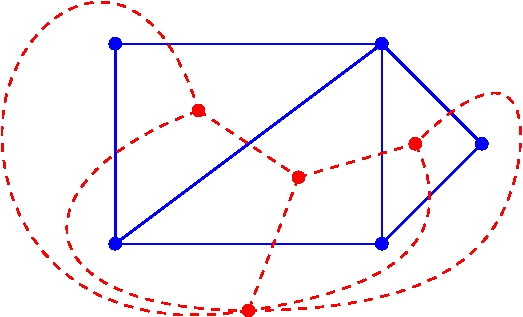
\includegraphics[height=130px]{Resources/Preliminaries-Dual.pdf}
	\caption{A plane graph $G$ (in blue) and its dual $G^*$ (in red).}
	\label{fig:preliminaries-dual}
\end{figure}

\Cref{fig:preliminaries-dual} illustrates an example of a plane graph and its dual.
Forming the dual of a plane graph essentially turns vertices into faces and vice versa and \quoted{rotates} the edges of the plane graph, as illustrated in \cref{fig:preliminaries-dual}.
Note that the planar embedding of the primal graph uniquely determines the embedding of its dual.
When forming the dual of the dual of a plane graph, we get back the original plane graph, \ie{}, $(G^*)^* = G$.



\paragraph{Contact Representations}

In a \emph{(simple) contact representation} of a plane graph $G_\phi$, the vertices are represented by pairwise internally disjoint regions of the plane, and edges are implicitly represented by the non-trivial contacts between the corresponding regions \cite{alam2013linear}.
Because $G_\phi$ is simple, the regions corresponding to adjacent vertices in $G_\phi$ must only share a single continuous boundary in the contact representation.
A contact representation is said to be \emph{hole-free} if all regions other than the unbounded outer region have a corresponding vertex in $G_\phi$.

Unless otherwise noted, we assume that contact representations are hole-free and that they respect the original graph $G_\phi$'s embedding; \ie{}, for all regions, the cyclic order of the boundaries with adjacent regions is equivalent to the cyclic order of the incident edges of the corresponding vertex in $G_\phi$ to its respective neighbors.

Given a plane graph $G_\phi$, a contact representation of $G_\phi$ with axis-aligned rectilinear polygons is called a \emph{rectilinear dual} of $G_\phi$ \cite{alam2013computing}.
The name \quoted{dual} is fitting here because vertices of the original graph turn into faces, or regions, of the rectilinear dual.
In fact, we can view the rectilinear dual as a plane graph itself: the polygons' corners are vertices connected by edges as determined by the polygons' sides, as illustrated in \cref{fig:preliminaries-rectilinear-dual}.
We use the term rectilinear dual to refer to the actual arrangement of rectilinear polygons and the induced plane graph interchangeably.

\begin{figure}[H]
	\centering
	\subfigure[]{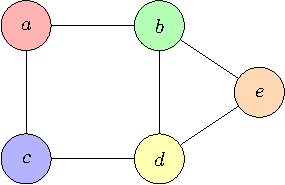
\includegraphics[height=90px]{Resources/Preliminaries-RectilinearDual-Primal.pdf}}
	\quad
	\subfigure[]{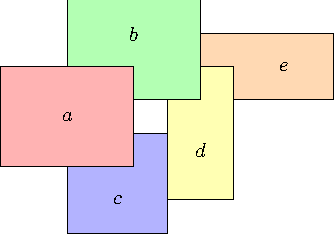
\includegraphics[height=90px]{Resources/Preliminaries-RectilinearDual-Polygons.pdf}}
	\quad
	\subfigure[]{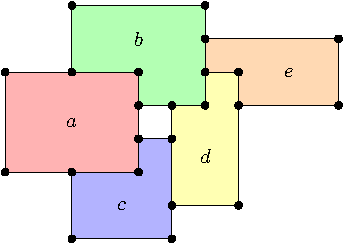
\includegraphics[height=90px]{Resources/Preliminaries-RectilinearDual-Dual.pdf}}
	\caption{A plane graph $G_\phi$ (a) and a possible rectilinear dual of $G_\phi$ with a hole, as a plain arrangement of polygons (b), and construed as yet another plane graph (c).}
	\label{fig:preliminaries-rectilinear-dual}
\end{figure}

A contact representation can be \emph{weighted}, assigning a real weight to all regions corresponding to vertices of its primal.
We define the \emph{normalized cartographic error} \cite{alam2015quantitative} of a weighted contact representation as
%
\begin{equation*}
    \max\limits_{v \in V(G)} \frac{\abs{A^\prime(v) - w(v)}}{\max\{A^\prime(v),w(v)\}},
\end{equation*}
%
where $w(v)$ is the prescribed area of the region corresponding to vertex $v$ and $A^\prime(v)$ is its actual area $A(v)$, normalized such that constant factors drop out, \ie{},
%
\begin{equation*}
	A^\prime(v) \coloneqq A(v) \cdot \frac{\sum\limits_{u \in V}{w(u)}}{\sum\limits_{u \in V}{A(u)}}.
\end{equation*}
%
We say that a weighted contact representation is \emph{$\varepsilon$-area-proportional} if its normalized cartographic error is less than or equal to $\varepsilon$.



\paragraph{Area Universality}

A plane graph $G$ with internal faces $F_\text{int}$ is \emph{area universal} if, for every area assignment of its internal faces $A \colon F_\text{int} \to \mathbb{R}_+$, there exists a planar straight-line drawing of $G$ with the same embedding such that all internal faces $f \in F_\text{int}$ have the area $A(f)$ prescribed by $A$.

Recall that Thomassen \cite{thomassen1992plane} showed that all (planar embeddings of) cubic graphs, \ie{}, graphs in which all vertices have degree 3, are area-universal, and that Kleist \cite{kleist2019planar} showed that all plane 1-subdivisions of planar graphs are area-universal, too.

\chapter{Visualizing Static Input Graphs}
\label{chap:visualizing-static-input-graphs}

In this chapter we provide a detailed description of our problem statement, formalize it, and discuss our solution in the case of static input graphs.

Our goal is to visualize clusters of a larger graph, such as an opinion network, as an artificial map.
In this map, each cluster of the larger graph is represented by a continuous region whose area is approximately proportional to the cluster's size, and neighboring regions indicate similarities between the respective clusters.

Unlike OpMap and GMap, which have similar goals, clustering the larger graph is not part of the framework we discuss here.
Instead, we assume the larger graph is clustered externally before being fed into our framework, producing some cluster graph.
The first step of our framework takes a spanning subgraph of this cluster graph as input and builds an initial contact representation in which all regions are simple polygons.
Obviously, this isn't possible for all spanning subgraphs of the cluster graph; for example, the subgraph must be planar.
We formalize the additional requirements we impose on the spanning subgraph in a bit.
The contact representation is then tweaked, displacing the polygons' corners in such a way that their areas are approximately proportional to the clusters' weights and they have somewhat organic shapes.
To formalize this, we require two short definitions:

\begin{definition}
A contact representation in which all regions are simple polygons is called a \emph{polygonal contact representation}.
\end{definition}

\begin{definition}
Given a plane graph $G$, a polygonal contact representation of $G$ is called a \emph{polygonal dual} of $G$.
\end{definition}

Note that polygonal duals are a generalization of rectilinear duals and that, analogous to rectilinear duals, a polygonal dual can be interpreted as plane graph itself: the polygons' corners translate to vertices in this graph, and their sides translate to edges.

\newcommand{\clustergraph}[1]{\ensuremath{G^\mathcal{C}_{#1}}}
\newcommand{\initmap}[1]{\ensuremath{\Gamma^*_{#1}}}
\newcommand{\propmap}[1]{\ensuremath{\Gamma^\propto_{#1}}}

With these definitions in place, we can formalize the structure of our framework:
Our input is a biconnected and internally triangulated plane subgraph of a cluster graph that we call the \emph{filtered cluster graph} \clustergraph{}.
We start by forming an initial weighted polygonal dual of \clustergraph{}, the \emph{initial map} \initmap{}.
\initmap{} inherits its (face) weights from the vertices of \clustergraph{}.
We then turn \initmap{} into an $\varepsilon$-area-proportional, polygonal contact representation of \clustergraph{} for some small $\varepsilon > 0$, the \emph{$\varepsilon$-proportional map} \propmap{} of \clustergraph{}.
This is done by displacing the the contact representation \initmap{}'s vertices while preserving its planarity.
We implement this step using a force-directed algorithm.

\begin{figure}[H]
	\centering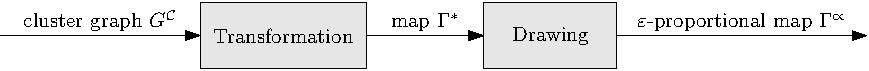
\includegraphics[width=0.9\textwidth]{Resources/Framework-1.pdf}
	\caption{Overview of the algorithmic pipeline for static input graphs.}
	\label{fig:static-pipeline-thesis}
\end{figure}

Let's break down the requirements we impose on the filtered cluster graph \clustergraph{}:

\begin{itemize}
\item \clustergraph{} is given as a plane graph.
Obviously, \clustergraph{} must be planar such that there exists a contact representation of \clustergraph{}.
We require a planar embedding of \clustergraph{} such that the \quoted{arrangement} of the clusters or of the regions on the eventual map is predetermined.
This becomes important in \cref{chap:visualizing-dynamic-input-graphs} where we start incorporating dynamic updates into the filtered cluster graph and resulting the map graphs.
\item \clustergraph{} must be internally triangulated such that the maps \initmap{} and \propmap{} are hole-free.
Applying the map metaphor, this translates to there not being any lakes or rivers separating countries on the map.
\cref{fig:preliminaries-rectilinear-dual} illustrates how internal faces on 4 or more vertices creates holes in contact representations.
\item \clustergraph{} must be biconnected such that, in combination with the internal triangulatedness, no vertex appears on the outer face multiple times.
The region of such a vertex in the polygonal dual would need to have multiple borders to the outer face, which we specifically excluded in \cref{chap:preliminaries}.
\item \clustergraph{} must be vertex-weighted such that the map \initmap{} can inherit its vertex weights and we know what areas the polygonal regions are supposed to have in \propmap{}.
\end{itemize}

Many real-world applications, such as visualizing opinion networks, do not produce a filtered cluster graph directly.
In order for our framework to be applicable, one may need to prepend a clustering phase that turns an arbitrary input graph $G$ into a biconnected and internally triangulated plane subgraph \clustergraph{} of a cluster graph of $G$ that can then be processed by our framework:
%
\begin{figure}[H]
	\centering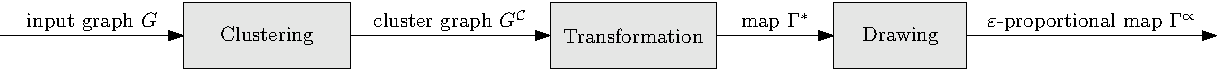
\includegraphics[width=0.9\textwidth]{Resources/Framework-2.pdf}
	\caption{Overview of a possible algorithmic pipeline for generic applications.}
	\label{fig:static-pipeline-application}
\end{figure}

We will now discuss our implementation of the transformation and drawing phases of the pipeline in detail.

\clearpage
\section{Transformation to Polygonal Dual}
\label{sect:transformation-to-dual}

In this step of the pipeline, we take a filtered cluster graph \clustergraph{} and form a polygonal dual of thereof, resulting in the map \initmap{}.
To formalize the their relationship, we need the concept of the augmented dual:

\begin{definition}
The \emph{augmented dual} $G^+$ of a plane graph $G$ is the plane multigraph obtained by first placing a new vertex $v^+$ in the outer face of $G$, connecting it to all vertices on the outer face, in order, without introducing edge crossings, and then forming its dual.
\label{def:augmented-dual}
\end{definition}

\Cref{fig:transformation-augmented-dual} illustrates how the augmented dual $G^+$ of a plane graph $G$ (\cref{subfig:transformation-augmented-dual-1}) is formed.
We add the helper vertex $v^+$ and helper edges $\{v^+,\cdot\}$ in the outer face in \cref{subfig:transformation-augmented-dual-2}.
We draw the helper edges as in \cite{wagner2016algorithmen} because it does not matter where in the plane this helper vertex lies \emdash{} all that matters is that each pair of adjacent vertices on the outer face forms a new triangular face with $v^+$.
In \cref{subfig:transformation-augmented-dual-3}, we overlay the dual vertices and edges in red.
\Cref{subfig:transformation-augmented-dual-4} shows just the augmented dual of $G$.
%
\begin{figure}[H]
	\centering
	\subfigure[]{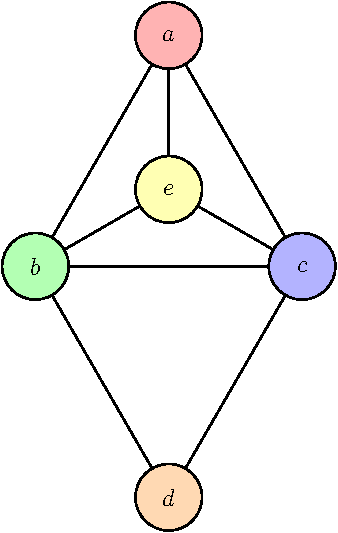
\includegraphics[height=130px]{Resources/Transformation-AugmentedDual-1.pdf}\label{subfig:transformation-augmented-dual-1}}
	\quad
	\subfigure[]{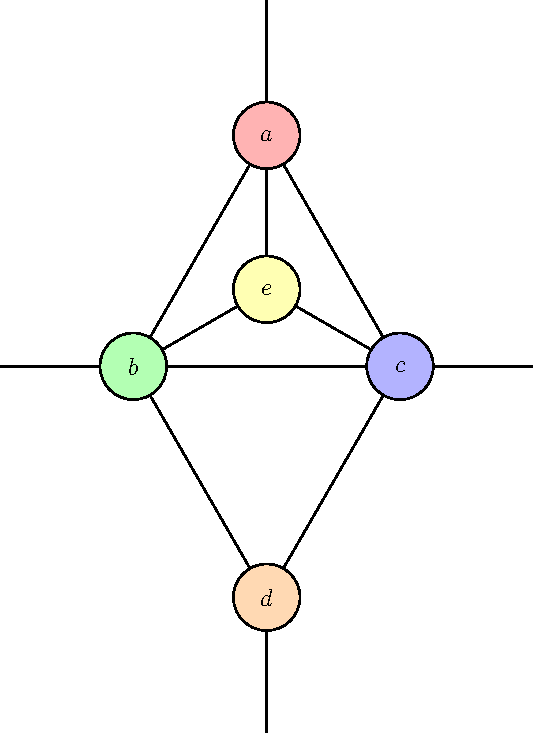
\includegraphics[height=130px]{Resources/Transformation-AugmentedDual-2.pdf}\label{subfig:transformation-augmented-dual-2}}
	\quad
	\subfigure[]{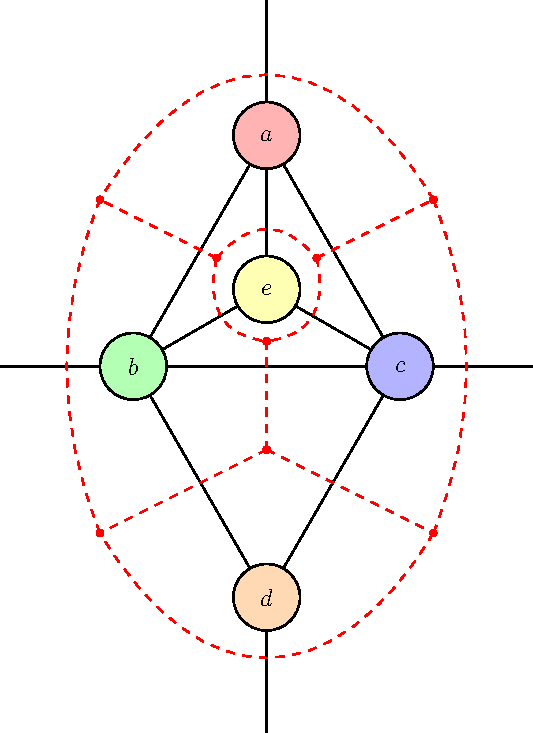
\includegraphics[height=130px]{Resources/Transformation-AugmentedDual-3.pdf}\label{subfig:transformation-augmented-dual-3}}
	\quad
	\subfigure[]{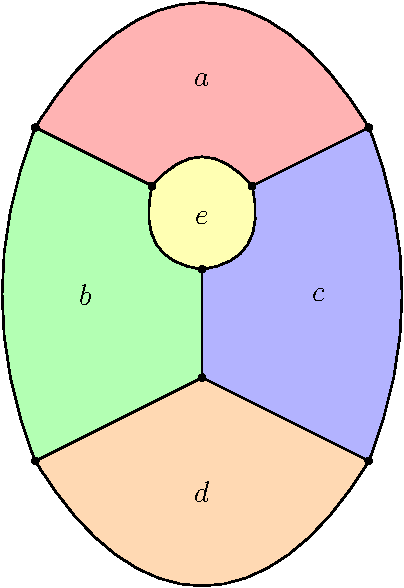
\includegraphics[height=130px]{Resources/Transformation-AugmentedDual-4.pdf}\label{subfig:transformation-augmented-dual-4}}
	\caption{Step-by-step representation of forming a plane graph's augmented dual.}
	\label{fig:transformation-augmented-dual}
\end{figure}

Note that analogous to the regular dual, the weak dual of the augmented dual of a plane graph $G$ is $G$ again, \ie{} $(G^+)^- = G$.

The augmented dual $G^+$ (\cref{subfig:transformation-augmented-dual-4}) of a biconnected and internally triangulated plane graph $G$ (\cref{subfig:transformation-augmented-dual-1}) essentially is a contact representation thereof.
In a polygonal dual, however, the edges cannot be curves and must be polylines instead.
The map \initmap{} can therefore be interpreted as a subdivision of the augmented dual $(\clustergraph{})^+$ in combination with a planar straight-line drawing thereof.



\paragraph{Algorithm Overview}

The underlying idea of creating the initial map \initmap{} is as follows:
Given a filtered cluster graph \clustergraph{}, we place vertices on edges of the outer face of \clustergraph{} (those edges bound additional triangular faces after adding the helper vertex in the process of forming the augmented dual) and inside the internal faces of \clustergraph{}.
We then connect these vertices if their corresponding faces are adjacent.
Connecting two vertices may require additional subdivision vertices or bends in order not to introduce edge crossings \emdash{} we use a single bend per edge.

The following figure illustrates an example:
%
\begin{figure}[H]
	\centering
	\subfigure[]{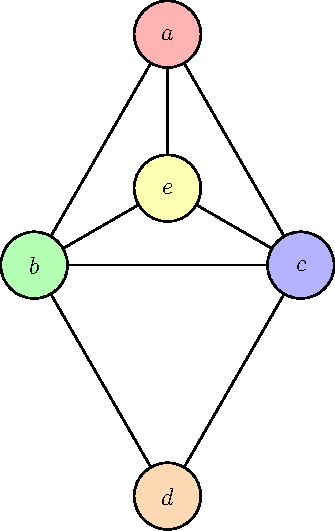
\includegraphics[height=70mm]{Resources/Transformation-Algorithm-1.pdf}\label{subfig:transformation-algorithm-1}}
	\quad
	\subfigure[]{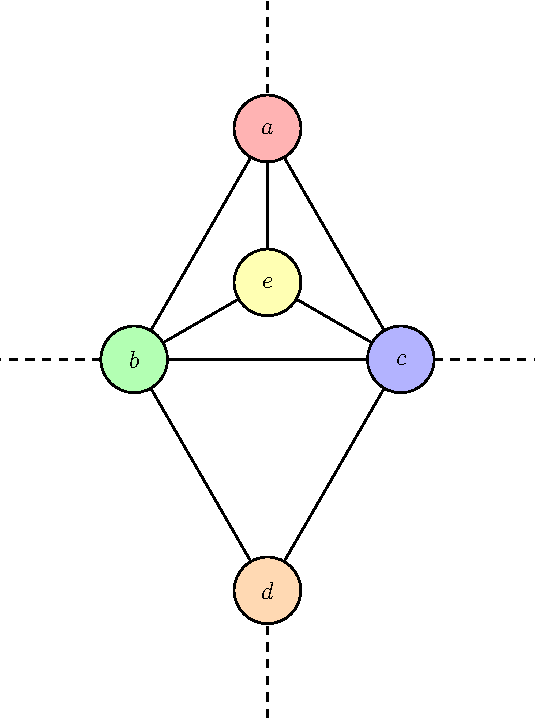
\includegraphics[height=70mm]{Resources/Transformation-Algorithm-2.pdf}\label{subfig:transformation-algorithm-2}}
	\quad
	\subfigure[]{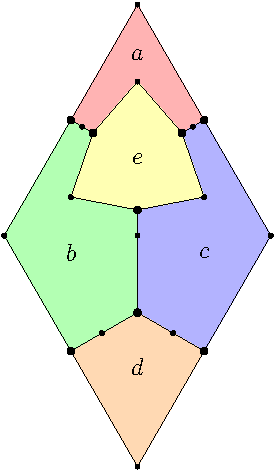
\includegraphics[height=70mm]{Resources/Transformation-Algorithm-3.pdf}\label{subfig:transformation-algorithm-3}}
	\caption{A filtered cluster graph \clustergraph{} (a), the helper graph \clustergraph{+} (b), and the polygonal dual \initmap{} of \clustergraph{} as produced by \cref{alg:transformation-to-dual} (c).}
	\label{fig:transformation-algorithm}
\end{figure}

Before feeding the filtered cluster graph \clustergraph{} into the algorithm, we construct a planar straight-line drawing \clusterdrawing{} of \clustergraph{} with the same planar embedding.
According to Fáry's theorem \cite{fary1948straight} \cite{wagner1936bemerkungen} \cite{stein1951convex}, such a drawing exists for every plane graph.
There are numerous popular algorithms to construct such a drawing, \eg{} Tutte's method \cite{tutte1963draw}, the shift method \cite{fraysseix1990draw}, or the Schnyder realizer method \cite{schnyder1990embedding}.



\clearpage
\paragraph{Algorithm Implementation}

\begin{algorithm}[H]
  \caption{Transformation to Polygonal Dual}
  \label{alg:transformation-to-dual}
  \SetKwData{Endpoints}{endpoints}
  \SetKwFunction{Appending}{appending}
  \SetArgSty{textrm}
  \vspace{5pt}
  \KwData{filtered cluster graph \clustergraph{} and a planar straight-line drawing \clusterdrawing{} thereof}
  \KwResult{polygonal dual \initmap{} of \clustergraph{}, in the form of a 1-subdivision of the augmented dual of \clustergraph{} and planar straight-line drawing thereof}
  \BlankLine
  create empty contact representation \initmap{}\;
  \BlankLine
  \tcp{compute dual vertices and edges}
  \ForEach{internal face $f$ in \clustergraph{}}{
    \label{line:transformation-loop1-start}
    add \quoted{internal face vertex} $v_f$ to \initmap{}\; \label{line:transformation-innerfacevertex}
    position $v_f$ at barycenter of $f$ in \clustergraph{} \label{line:transformation-barycenter1}\;
    \label{line:transformation-loop1-end}
  }
  \ForEach{edge $\{u,v\}$ in \clustergraph{}}{
    \label{line:transformation-loop2-start}
  	\If{$\{u,v\}$ is incident to two different internal faces $f, g$ in \clustergraph{} \label{line:transformation-incidentfacelookup1}}{
  	  add \quoted{subdivision vertex} $v_\text{sub}$ to \initmap{}\; \label{line:transformation-subdivisionvertex1}
  	  position $v_\text{sub}$ at midpoint of ${\{u,v\}}$ in \clustergraph{}\;
  	  add edge between $v_f$ and $v_\text{sub}$ to \initmap{}\; \label{line:transformation-edgetype1-start}
  	  add edge between $v_\text{sub}$ and $v_g$ to \initmap{}\; \label{line:transformation-edgetype1-end}
  	}
  	\ElseIf{$\{u,v\}$ is incident to a single internal face $f$ in \clustergraph{} \label{line:transformation-incidentfacelookup2}}{
  	  add \quoted{outer edge vertex} $v_{\{u,v\}}$ to $G_\text{init}$\; \label{line:transformation-outeredgevertex}
  	  position $v_{\{u,v\}}$ at midpoint of ${\{u,v\}}$ in \clustergraph{}\;
  	  add \quoted{subdivision vertex} $v_\text{sub}$ to \initmap{}\; \label{line:transformation-subdivisionvertex2}
  	  position $v_\text{sub}$ at midpoint of segment between barycenter of $f$ and midpoint of ${\{u,v\}}$ in \clustergraph{} \label{line:transformation-barycenter2}\;
  	  add edge between $v_{\{u,v\}}$ and $v_\text{sub}$ to \initmap{}\; \label{line:transformation-edgetype2-start}
  	  add edge between $v_\text{sub}$ and $v_f$ to \initmap{}\; \label{line:transformation-edgetype2-end}
  	}
  	\label{line:transformation-loop2-end}
  }
  \ForEach{incident edges $\{\{u,v\},\{v,w\}\}$ on outer face of \clustergraph{}}{
    \label{line:transformation-loop3-start}
    add \quoted{subdivision vertex} $v_\text{sub}$ to \initmap{}\; \label{line:transformation-subdivisionvertex3}
    position $v_\text{sub}$ at position of $v$ in \clustergraph{}\;
    add edge between $v_{\{u,v\}}$ and $v_\text{sub}$ to \initmap{}\; \label{line:transformation-edgetype3-start}
    add edge between $v_\text{sub}$ and $v_{\{v,w\}}$ to \initmap{}\; \label{line:transformation-edgetype3-end}
    \label{line:transformation-loop3-end}
  }
  \BlankLine
  \tcp{compute faces in \initmap{} and match them to vertices in \clustergraph{}}
  \ForEach{vertex $u$ in \clustergraph{} \label{line:transformation-enumeratevertices}}{
    \label{line:transformation-loop4-start}
    $\Endpoints \gets ()$\;
    \ForEach{adjacent pair $(v,w)$ of neighbors of $u$ in counterclockwise order \label{line:transformation-enumerateedges}}{
      \If{$(u,v,w)$ bound a triangular face $f$ in counterclockwise order in \clustergraph{} \label{line:transformation-checktriangle}}{
        append $v_f$ to \Endpoints\;
      }
      \Else{
        append $v_{\{u,v\}}$ to \Endpoints\;
        append $v_{\{u,w\}}$ to \Endpoints\;
      }
    }
    \ForEach{adjacent pair $(v,w)$ in \Endpoints \label{line:transformation-insertsubdivisions}}{
      insert subdivision vertex connecting $v$ to $w$ between $v$ and $w$ in \Endpoints\;
    }
    define $f_u$ as internal face on \Endpoints in \initmap{}\;
    set weight of $f_u$ in \initmap{} to weight of $u$ in \clustergraph{}\;
    \label{line:transformation-loop4-end}
  }
  \Return \initmap{}
\end{algorithm}
\vfill



\paragraph{Algorithm Correctness}

We show the algorithm's correctness in two steps.
First, we show that the algorithm does indeed construct a 1-subdivision of the augmented dual of \clustergraph{}.
Second, we show that the constructed drawing thereof is planar, making it a contact representation of \clustergraph{} as previously explained and illustrated in \cref{fig:transformation-augmented-dual}.

Recall that $(\clustergraph{})^+$ is a contact representation of \clustergraph{}.
We can construct $(\clustergraph{})^+$ via a helper graph \clustergraph{+} that we obtain by inserting a helper vertex $v^+$ in the outer face of \clustergraph{} and connecting it to all vertices on the outer face of \clustergraph{}, in order, without introducing edge crossings.
The contact representation $(\clustergraph{})^+$ then is the regular dual of \clustergraph{+}, \ie{} $(\clustergraph{})^+ = (\clustergraph{+})^*$.
By adding the helper vertex $v^+$ and helper edges $\{v^+,\cdot\}$, the edges on the outer face of \clustergraph{} bound new triangular faces of \clustergraph{+}.

The dual of a plane graph has vertices in each of the primal graph's faces.
We place these vertices in the original internal faces in \cref{line:transformation-innerfacevertex} and in \emdash{} or rather on \emdash{} the new triangular faces in \clustergraph{+} in \cref{line:transformation-outeredgevertex}.
Vertices in the dual are adjacent if their respective faces are adjacent in the primal.
Thus for every edge separating two faces in the primal \clustergraph{+}, we require a dual edge in $(\clustergraph{+})^*$.
We add these edges in \crefrange{line:transformation-edgetype1-start}{line:transformation-edgetype1-end} (for adjacent internal faces in \clustergraph{}), in \crefrange{line:transformation-edgetype2-start}{line:transformation-edgetype2-end} (for edges separating an internal face in \clustergraph{} from a new face in \clustergraph{+}), and in \crefrange{line:transformation-edgetype3-start}{line:transformation-edgetype3-end} (for helper edges $\{v^+,\cdot\}$ separating two new faces in \clustergraph{+}).
Because we place all bends of the dual edges on the respective primal edge, the cyclic order of the edges incident to each vertex is equivalent to the cyclic order of the edges bounding the respective faces in the primal.

\begin{figure}[H]
	\centering
	\subfigure[]{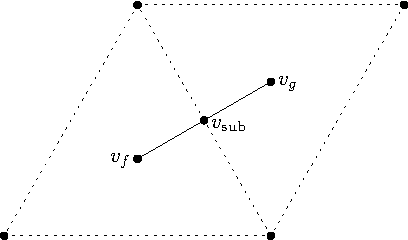
\includegraphics[height=32mm]{Resources/Transformation-DualEdgeConstruction-1.pdf}\label{subfig:transformation-dual-edge-construction-1}}
	\subfigure[]{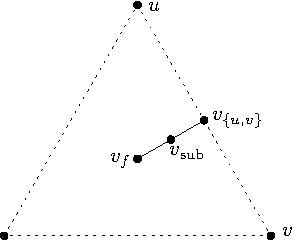
\includegraphics[height=32mm]{Resources/Transformation-DualEdgeConstruction-2.pdf}\label{subfig:transformation-dual-edge-construction-2}}
	\quad
	\subfigure[]{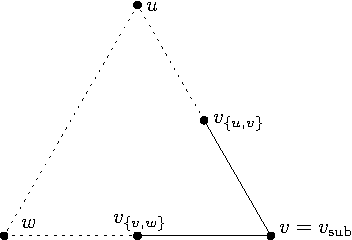
\includegraphics[height=32mm]{Resources/Transformation-DualEdgeConstruction-3.pdf}\label{subfig:transformation-dual-edge-construction-3}}
	\caption{Construction of the dual edges as per \cref{alg:transformation-to-dual} between two internal faces in \clustergraph{} (a), between an internal face of \clustergraph{} and a new face in \clustergraph{+} (b), and between two new faces in \clustergraph{+} (c). The dotted lines are edges in \clustergraph{}.}
	\label{fig:transformation-dual-edge-construction}
\end{figure}

It is left to show that the placement of vertices and edges produces a crossing-free drawing.
To do so, we consider the edges from non-subdivision vertices in $(\clustergraph{+})^*$ to their neighbors.
Recall that those vertices correspond to faces in \clustergraph{+}.
Following the construction illustrated in \crefrange{subfig:transformation-dual-edge-construction-1}{subfig:transformation-dual-edge-construction-2}, the three incident edges to a vertex corresponding to an internal face of \clustergraph{} lie completely inside said face.
Because these edges go straight towards the midpoint of the incident edges, they don't self-intersect.

The vertices corresponding to new faces in \clustergraph{+} lie on the midpoint of the bounding edge that already exists in \clustergraph{}.
The dual edges connecting two of those vertices are constructed such that they partition the boundary of the outer face of \clustergraph{} (see \cref{subfig:transformation-dual-edge-construction-3}) and therefore don't intersect any of the edges discussed so far.
Their edge to the vertex corresponding to the adjacent internal face goes straight towards said vertex, meeting it halfway, as illustrated in \cref{subfig:transformation-dual-edge-construction-2}.
Because some $v_f$'s incident edges all go straight towards its bounding edges as outlined above, this kind of edge does not introduce any edge crossings either.
The constructed graph and drawing is therefore a 1-subdivision of the augmented dual of \clustergraph{} and the drawing is planar.

Once the algorithm has constructed \initmap{}, we compute an explicit representation of its internal faces and the corresponding vertices in the primal.
We do so for the augmented dual $(\clustergraph{})^+$ first (loop in \cref{line:transformation-enumerateedges}) and then insert the subdivision vertices (loop in \cref{line:transformation-insertsubdivisions}).
The face in $(\clustergraph{})^+$ that corresponds to a vertex $v$ of \clustergraph{} is bounded by vertices corresponding to internal faces of \clustergraph{} that contain $v$, plus the vertices corresponding to the additional triangular faces in \clustergraph{+} in case $v$ lies on outer face of \clustergraph{}.
Iterating over adjacent pairs $(e_1, e_2)$ of incident edges in counterclockwise order correctly detects the internal faces between $e_1$ and $e_2$ and the case where $e_1$ and $e_2$ wrap around on the outside, in order.
The orientation check in \cref{line:transformation-checktriangle} is required such that the wraparound case isn't misclassified as an internal face.
This would be the case for internal faces of \clustergraph{} with two edges on the outer face, as is the case for vertex $v \coloneqq d$ and edges $e_1 \coloneqq \{d,b\}, e_2 \coloneqq \{d,c\}$ in \cref{fig:transformation-algorithm}.



\paragraph{Algorithm Runtime}

To compute the input graph's faces, we replace every edge with two inversely oriented, directed edges.
We then repeatedly pick any unmarked edge and form a directed cycle by following the next outgoing edge according to the embedding, marking the edges as we go.
Once all edges have been marked, we have found all faces.
The outer face is the one face whose interior is on the left when traveling along its bounding edges.
This can be implemented in $\bigTheta{n+m}$, where $n = \lvert V(\clustergraph{}) \rvert$ and $m = \lvert E(\clustergraph{}) \rvert$.

The input graph has $\bigTheta{n}$ internal faces and they are all triangles, therefore we can compute their barycenter in $\bigTheta{1}$ each (\cref{line:transformation-barycenter1}, \cref{line:transformation-barycenter2}).
By keeping track of of which faces an edge of the input graph is incident to while computing the faces as outlined above, we allow for $\bigTheta{1}$ lookups in \cref{line:transformation-incidentfacelookup1} and \cref{line:transformation-incidentfacelookup2}.
The loop in \crefrange{line:transformation-loop1-start}{line:transformation-loop1-end} therefore runs in $\bigTheta{n}$, the loop in \crefrange{line:transformation-loop2-start}{line:transformation-loop2-end} in $\bigTheta{m}$, and the loop in \crefrange{line:transformation-loop3-start}{line:transformation-loop3-end} in $\bigTheta{m}$.

The loop in \crefrange{line:transformation-loop4-start}{line:transformation-loop4-end} processes every vertex once in \cref{line:transformation-enumeratevertices} and and every edge twice \cref{line:transformation-enumerateedges}.
We can check if the vertices $u,v,w$ form a triangle in constant time (\cref{line:transformation-checktriangle}) by checking if there's an edge between $v$ and $w$.
Considering each of the $\bigTheta{n+m}$ vertices of the generated graph appears in \code{endpoints} in no more than two iterations of the loop in \crefrange{line:transformation-loop4-start}{line:transformation-loop4-end} and all those vertices have degree 3, we can find their shared neighbor in constant time and implement the entire loop to run in $\bigTheta{n+m}$.

The entire algorithm can therefore be implemented to run in $\bigTheta{n+m}$.



\paragraph{Theoretical Bounds}

But do we have to subdivide edges of the augmented dual of our filtered cluster graph \clustergraph{} in order to get a valid polygonal dual of \clustergraph{}?
Although the augmented dual $(\clustergraph{})^+$ is plane by definition, it is not immediately obvious that there exists a planar straight-line drawing of $(\clustergraph{})^+$ \emdash{} and that's what we need for it to be a polygonal contact representation.

In our case, however, $(\clustergraph{})^+$ is simple, \ie{} there are no loops or multiple adjacencies.
Recall that \clustergraph{} is biconnected and internally triangulated.
Adding the helper vertex in the outer face of \clustergraph{} and connecting it to all vertices on the outer face therefore creates a fully triangulated, simple graph.
In a simple triangulated graph, there are no two edges that are incident to the same faces (only those would create multiple adjacencies when forming the dual) and no edges that have the same face on both sides (only those would create loops when forming the dual) either.
The augmented dual $(\clustergraph{})^+$ is therefore simple and, according to Fáry's theorem \cite{fary1948straight}, there exists a planar straight-line drawing of $(\clustergraph{})^+$ respecting its original planar embedding.

In addition to having a planar straight-line drawing, $(\clustergraph{})^+$ is also a cubic graph, \ie{} one in which all vertices have degree 3.
This is because \clustergraph{} with the helper vertex is a triangulated graph, meaning every face is incident to exactly three edges, which turns into every vertex being incident to exactly three edges when forming the dual.
According to the results of Thomassen \cite{thomassen1992plane}, $(\clustergraph{})^+$ is therefore area-universal.
This means that regardless of the concrete face weights that \clustergraph{} prescribes, there exists a planar straight-line drawing of $(\clustergraph{})^+$ realizing those weights/areas.

Even without subdividing edges in $(\clustergraph{})^+$, we could therefore choose the map \initmap{} in such a way that it has perfect statistical accuracy already.
Such a drawing of $(\clustergraph{})^+$ is non-trivial to compute though and creates undesired region shapes according to our other quality metrics.
Instead, the algorithm we proposed here subdivides all edges of the augmented dual $(\clustergraph{})^+$ once and leaves us with a decent initial drawing and enough degrees of freedom to optimize for other quality metrics in \cref{sect:drawing-the-dual}.


\clearpage
\section{Drawing the Polygonal Dual}
\label{sect:drawing-the-dual}

In the second step of the pipeline, we apply a force-directed graph drawing algorithm to the initial map graph $G_\text{init}$ produced by \cref{alg:transformation-to-dual} to generate the approximately area-proportional map graph $G_\text{prop}$.

In a force-directed algorithm, we interpret a graph's vertices as particles in a physical system.
Based on the structure of the graph and the relative position of the particles, we define several forces that act to bring the system to a stable equilibrium position in which its potential energy is at a local minimum.
In these equilibrium positions, the system is in a somewhat relaxed state that, in the context of graph drawing, generally is a visually appealing drawing of the graph.
We find an equilibrium position by iteratively computing the net force acting on each particle and displacing it by a small amount in the direction of the net force, based on its absolute value.



\paragraph{Forces}

%https://slideplayer.com/slide/4924642/
%v-v-rep: Eades 1984, Fruchterman & Reingold
%v-e-rep: Davidson & Harel 1996, Bertault 1999

We define the forces that exist in our particle system with two goals in mind:
First, the faces of the graph (the regions of the map) to have an area ought to be close to proportional to some prescribed value.
Second, we want the faces to be \emph{locally fat}.
Our intuitive understanding of local fatness is that a region shouldn't have drawn-out, tight corridors.
We formalize and discuss different quantifiable measures that aim to capture the local fatness of regions in \cref{chap:evaluation}.
Note that both of these are soft requirements.
Planarity of the resulting drawing, on the other hand, is a hard requirement that must be preserved at all costs.

Let us now discuss the concrete force components that act to bring our particle system to an equilibrium position.
%
\begin{itemize}
\item \textbf{Air Pressure:} % alam2013computing
Motivated by Alam \etal{} \cite{alam2013computing}, we treat the polygonal regions as volumes of some amount of air equal to the respective face's weight.
This allows us to define an analog to air pressure in the polygonal regions that exerts forces on the regions' edges.
This force is responsible for growing faces that are currently compressed and shrinking faces that are currently larger than they should be, therefore working towards the statistical accuracy of the generated map.

We want this force and the overall drawing to be agnostic to constant factors of the face weights and therefore compute the normalized pressure $P(f)$ in an internal face $f$ as
%
\begin{equation*}
	P(f) \coloneqq \frac{w(f)}{A(f)} \cdot \frac{\sum_{g \in F}{A(g)}}{\sum_{g \in F}{w(g)}},
\end{equation*}
%
where $A(f)$ is the area currently covered by some internal face $f$ and $w(f)$ its weight.
We set the normalized pressure in the outer face to the weighted average normalized pressure, \ie{}
%
\begin{equation*}
	P(f_\text{outer}) \coloneqq \frac{\sum_{f \in F}{A(f) \cdot P(f)}}{\sum_{f \in F}{A(f)}} = 1.
\end{equation*}

Physical pressure is the ratio of force to area.
The air pressure in each of the regions $f$ therefore exerts a force on each bounding edge $e = \{u,v\}$ based on the pressure's magnitude and the edge's length $l(e)$ in relation to the entire region's boundary's length $l(f)$.
We orient $e = \{u,v\}$ such that $u$ directly precedes $v$ on the boundary of $f$ and define the force as
%
\begin{equation}
	\vec{F}_P((u,v);f) \coloneqq
	3 \cdot P(f)\cdot\frac{l(e)}{l(f)}
	\cdot \Norm(\Perp(\longvec{vu}))
	,
\end{equation}
%
where $\Perp(\cdot)$ rotates a vector by $90^\circ$ in counterclockwise direction and $\Norm(\cdot)$ normalizes a vector to unit length.
We apply $\vec{F}_P(\{u,v\};f)$ to both endpoints $u$ and $v$ of the edge, as illustrated in \cref{fig:drawing-forces-air-pressure}.

\begin{figure}[H]
	\centering
	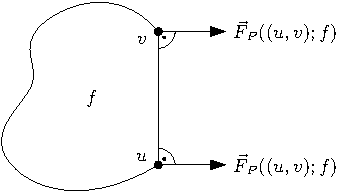
\includegraphics[height=35mm]{Resources/Drawing-Forces-AirPressure.pdf}
	\caption{Forces exerted on the endpoints of the edge $e = \{u,v\}$ by the air pressure in the region $f$.}
	\label{fig:drawing-forces-air-pressure}
\end{figure}

Considering every edge is incident to exactly two faces, we can write the net force exerted on an oriented edge $e = (u,v)$ incident to face $f$ on the left and face $g$ on the right as
%
\begin{equation*}
	\vec{F}_P((u,v);f,g) \coloneqq
	3 \cdot \left( P(g)\cdot\frac{l(e)}{l(g)} - P(f)\cdot\frac{l(e)}{l(f)} \right)
	\cdot \Norm(\Perp(\longvec{uv}))
	,
\end{equation*}
%
matching the force that Alam \etal{} \cite{alam2013computing} use for computing their cartograms.


\item \textbf{Angular Resolution:} % argyriou2013maximizing
Internal face angles close to $0^\circ$ cause tight corridors in the form of pointy spikes and angles close to $360^\circ$ the opposite \emdash{} both features we want to avoid if possible.
We therefore define a force that optimizes angular resolution, \ie{} a force that tries to evenly distribute the angles formed by the incident edges around a vertex $v$ at $\frac{360^\circ}{\deg(v)}$ each.

Let $v$ be a vertex and let $u$ and $w$ be two successive neighbors of $u$ in counterclockwise order.
Also let $\measuredangle_{uvw} \in \lbrack 0^\circ, 360^\circ )$ denote the normalized angle from $u$ via $v$ to $w$ measured in counterclockwise direction.
%Analogous to \cite{argyriou2013maximizing}, we define an angular force
With this, we define the force $\vec{F}_\measuredangle(v;u,w)$ as
%
\begin{equation}
	\vec{F}_\measuredangle(v;u,w) \coloneqq
	\frac{1}{2} \cdot \frac{\frac{360^\circ}{\deg(u)} - \measuredangle_{uvw}}{\measuredangle_{uvw}}
	\cdot \Bsc(\angle_{uvw})
	.
\end{equation}

Here $\Bsc(\angle_{uvw})$ computes the normalized bisector of the given angle, \ie{} $\Norm(\longvec{vu})$ rotated by $\frac{1}{2} \measuredangle_{uvw}$ in counterclockwise direction.
The construction of $\vec{F}_\measuredangle(v;u,w)$ is illustrated in \cref{fig:drawing-forces-angular-resolution}.

\begin{figure}[H]
	\centering
	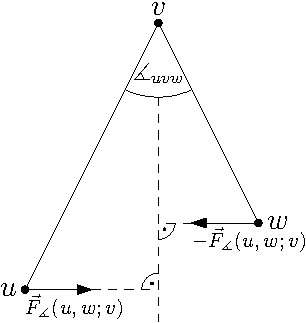
\includegraphics[height=40mm]{Resources/Drawing-Forces-AngularResolution.pdf}
	\caption{Force exerted on some vertex $v$ with successive neighbors $u$ and $w$ of $v$ where $\measuredangle_{uvw} > \frac{360^\circ}{\deg(v)}$.}
	\label{fig:drawing-forces-angular-resolution}
\end{figure}

For all triplets $(u,v,w)$ of vertices $v$ and successive neighbors $u$, $w$ of $v$, we apply $\vec{F}_\measuredangle(v;u,w)$ to $v$.
If the angle at $v$ is currently too small, the force acts to move $v$ along the bisector, thereby increasing the angle; otherwise it acts to move $v$ against the bisector, thereby decreasing the angle.

Argyriou \etal{} \cite{argyriou2013maximizing} use a similar force to obtain uniform angles around all vertices.
However, instead of applying the force to the vertex $v$ whose angular resolution we want to improve as we do, they apply perpendicular forces to its neighbors.
In our tests, the approach of Argyriou \etal{} has shown not to converge well due to us not having a force acting towards a uniform edge length, as discussed below in a bit.


\item \textbf{Vertex-vertex repulsion:} % eades84heuristic
We define a repulsive force between pairs of vertices to prevent the vertices from clumping together.
This is important because in order to preserve planarity, vertices that are very close to others will need to have their movement restricted severely, possibly hindering us from satisfying our aesthetic criteria.
We think of the vertices as charged particles that push each other away and define a repulsive force based on Coulomb's law that is exerted along the line connecting pairs of vertices and whose magnitude depends on their Euclidean distance:
%
\begin{equation}
	\vec{F}_\leftrightarrow(u;v) \coloneqq
	25 \cdot \frac{1}{\norm{\longvec{uv}}^2}
	\cdot \Norm(\longvec{uv})
\end{equation}

For pairs $(u, v) \in V^2, u \neq v$, we apply $\vec{F}_\leftrightarrow(u;v)$ to $u$.
We restrict ourselves to pairs $(u,v)$ where $u$ and $v$ lie together on the boundary of some face for performance reasons and because for other pairs, there'd be other vertices or edges between $u$ and $v$ that would push the two vertices apart.

This kind of force was first used by Eades \cite{eades84heuristic}, albeit only for non-adjacent pairs of vertices.
We apply this force to adjacent vertices as well because we don't use spring-like forces between adjacent vertices trying to achieve a uniform edge length (and therefore some non-zero distance) as Eades does, as discussed below.


\item \textbf{Vertex-edge repulsion:} % bertault1999force
In another attempt to prevent tight corridors from forming, we define an additional repulsive force between vertices and edges.
Given an edge $e = \{u,w\}$ and non-incident vertex $v$, we define $v_+$ as the point on the segment from $u$ to $w$ with the smallest Euclidean distance to $v$.
We then define the repulsive force as
%
\begin{equation}
	\vec{F}_\bot(v;\{u,w\}) \coloneqq
	10 \cdot \frac{1}{\norm{\longvec{v_+v}}^2}
	\cdot \abs{\vec{n}_e \cdot \Norm(\longvec{v_+v})}
	\cdot \Norm(\longvec{v_+v})
	,
\end{equation}
%
where $\vec{n}_e$ is the normalized normal vector of the edge $e$ pointing in either direction.
The following figure illustrates the construction of the force $\vec{F}_\bot(v;\{u,w\})$:
%
\begin{figure}[H]
	\centering
	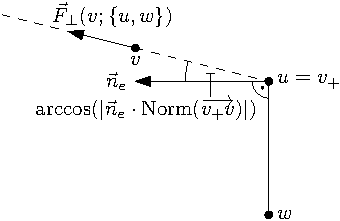
\includegraphics[height=40mm]{Resources/Drawing-Forces-VertexEdgeRepulsion.pdf}
	\caption{Force exerted on some vertex $v$ by a non-incident edge $\{u,w\}$.}
	\label{fig:drawing-forces-vertex-edge-repulsion}
\end{figure}

Analogous to the vertex-vertex-repulsion discussed above, we compute the force $\vec{F}_\bot(v;\{u,w\})$ only for vertices and edges that lie together on the boundary of some face and apply it to $v$.

This repulsive force is very similar to what Bertault uses in PrEd \cite{bertault1999force}.
However, we have an additional dot product term for how $v$ is positioned relatively to the edge $\{u,w\}$ whereas Bertault drops the force altogether if the orthogonal projection of $v$ onto the line through $u$ and $w$ doesn't lie between $u$ and $w$.
In our tests, Bertault's definition resulted in very unstable simulations as these force swayed back and forth between having full impact and no impact at all.
\end{itemize}

The constant factors of the force components above were determined experimentally and yielded good results for a variety of randomly generated graphs.

Note that we do not define attractive forces between adjacent vertices as most traditional force-directed algorithms do.
Such an attractive force is generally used to keep adjacent vertices close together while nonadjacent vertices are pushed further apart by the repulsive forces.
This works for many graph drawing algorithms because for them, uniform edge length is a desired feature in equilibrium.
In our case, however, there is no correlation between the extent of a region and the number of edges on its boundary and, subsequently, the length of the edges on its boundary.
Including such an attractive force here would in fact be counterproductive.

To make sure that the physical simulation converges, we cool the particle system down over time.
We define a global cooling parameter $\alpha = 0.01$ and, at step $i$ of the iterative process, add $(1 - \alpha)^i$ as a factor to all of the forces mentioned above.
By doing so, we prevent unstable oscillations around equilibrium.

In our implementation, we also smooth vertices of degree 2 that become too close to other vertices and subdivide edges that become too long in order to create more degrees of freedom in the respective face's shape.
To do so, we first compute the average edge length $\bar{l}$ as
%
\begin{equation*}
	\bar{l} \coloneqq \frac1{\abs{E}} \cdot \sum\limits_{e \in E} l(e)
	.
\end{equation*}
%
Then, at each iteration, we subdivide edges that are longer than $2\bar{l}$ at their midpoint and smooth vertices whose distance to the closest other vertex is $\frac{1}{10}\bar{l}$ or less if we can do so without introducing edge crossings.



\paragraph{Preventing Edge Crossings}

When iteratively displacing the map graph's vertices according to the forces defined above, we must pay close attention to not accidentally introduce edge crossings.

To do so, we adopt the rules of ImPrEd \cite{simonetto2011impred} that ensure no edge crossings are created.
At each step of the algorithm, ImPrEd computes the maximum distance each of the vertices is allowed to move such that the drawing's edge crossing properties are guaranteed to be preserved.
The maximum displacement per vertex is computed in eight general directions, zones of $45^\circ$ each.
The actual displacement of the vertices is then clamped at the maximum distance the vertex can safely move in the desired direction.


\chapter{Visualizing Dynamic Input Graphs}
\label{chap:visualizing-dynamic-input-graphs}

Extending the approach discussed in the previous section to dynamic input graphs is challenging primarily because we must try to preserve the viewer's mental map as the underlying data changes over time.
We want the visualization at different points in time to be similar enough so that the viewer can clearly tell what parts have changed \cite{mashima2011visualizing}, yet allow for the required changes in geography and topology.
Still, changes between visualizations at consecutive points in time should minimize movement and allow for smooth animations therebetween.

Extending the pipeline for static inputs discussed in the previous section in a straightforward way will not satisfy these requirements.
Running through the entire pipeline with a different, albeit similar, input graph, may result in a completely different visualization, destroying the viewer's mental map.
This is because even though the combinatorial arrangement of the regions of the map \propmap{t} is predetermined by the planar embedding of the filtered cluster graph \clustergraph{t}, the independent nature of the runs through the pipeline can result in regions with drastically different shapes and (absolute) positions.
We therefore extend the pipeline in a way that allows for small, incremental changes to be propagated through the pipeline and to eventually be applied to the previous output in a way that preserves the viewer's mental map.

We extend the pipeline for static input by an incremental transformation phase.
This phase takes two inputs:
A map \initmap{t} that the pipeline previously produced as output for some filtered cluster graph \clustergraph{t}, and a sequence of operations on said cluster graph, that, when applied to \clustergraph{t}, yields the cluster graph \clustergraph{t+1}.
The incremental transformation phase then determines how these operations translate to a polygonal dual of \clustergraph{t} and applies the translated operations to \initmap{t}, producing \initmap{t+1}, a polygonal dual of \clustergraph{t+1}.
This new polygonal dual is then fed back into the drawing phase to make it an $\varepsilon$-area-proportional contact representation \propmap{t+1} for some small $\varepsilon > 0$ and to improve the local fatness of the map's regions.

\begin{figure}[H]
	\centering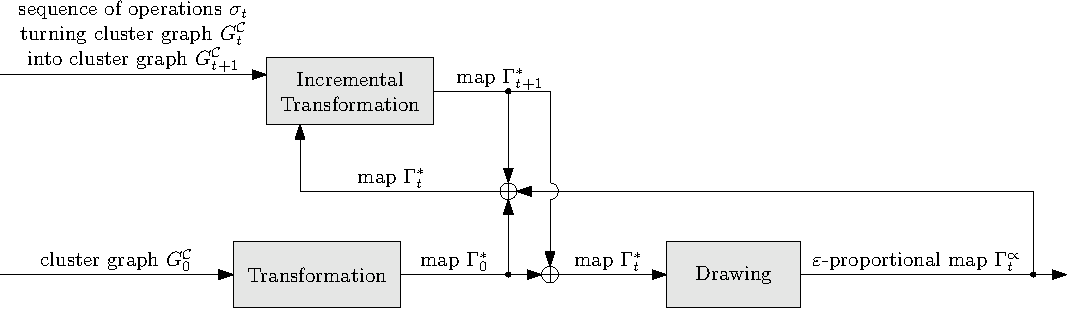
\includegraphics[width=0.9\textwidth]{Resources/Framework-3.pdf}
	\caption{Overview of the algorithmic pipeline for dynamic input graphs.}
	\label{fig:dynamic-pipeline-thesis}
\end{figure}

Real-world applications, such as visualizing a dynamic opinion network, need a way to feed a sequence of operations on the filtered cluster graph into our framework.
This could be done by prepending an incremental clustering phase that translates changes to the simple input graph $G_t$ into changes of its filtered cluster graph \clustergraph{t}.
However, such a sequence of operations $\sigma_t$ is only meaningful in combination with a graph that these operations can be applied to.
One must therefore provide the previously-produced cluster graph \clustergraph{t} as additional input to the incremental clustering phase such that it can tailor its output to the cluster graph that has already been locked in in an earlier run through the pipeline.
This possible extension to our pipeline is illustrated in the following figure:
%
\begin{figure}[H]
	\centering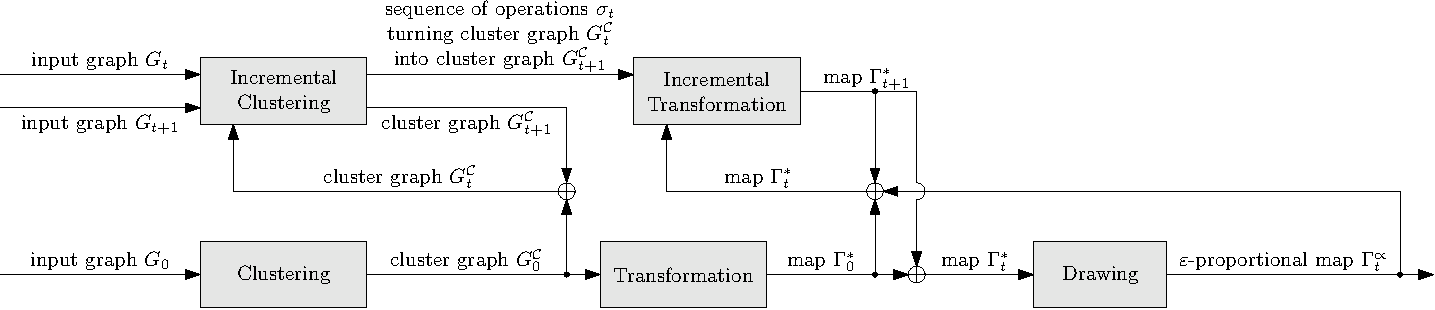
\includegraphics[width=\textwidth]{Resources/Framework-4.pdf}
	\caption{Overview of a possible algorithmic pipeline for generic applications.}
	\label{fig:dynamic-pipeline-application}
\end{figure}

Extending the pipeline to allow the propagation of small, incremental changes of the input graph has numerous benefits other than the ability to preserve the viewer's mental map:
%
\begin{itemize}
\item It allows highly efficient implementations of the incremental parts of the pipeline as only the aspects that have actually changed in the input graph or intermediate products need to be processed and propagated further along the pipeline.
\item It makes the pipeline highly parallelizable for dynamic inputs: when a later phase is processing changes, an earlier phase can already start processing new changes independently.
With our force-directed implementation of the drawing phase, we can even incorporate dynamic updates while the drawing phase is still running, even if it has not converged yet: we pause the force simulation, feed the current map \initmap{t} into the incremental transformation phase to incorporate the dynamic updates, and then resume the simulation with the updated map graph \initmap{t+1} produced by the incremental transformation phase.
\item It efficiently supports dynamic input in an online setting, \ie{} a setting in which the incremental changes aren't known in advance, for example when visualizing live data.
\end{itemize}



\paragraph{Supported Operations}

Our pipeline supports numerous classes of atomic operations on the filtered cluster graph, such as inserting and removing vertices and edges, flipping edges, or simply changing a cluster's weight.
By composing multiple atomic operations in a sequence, more drastic changes can be made to the filtered cluster graph.
In our pipeline, the operations are applied one after the other nonetheless.

The simplest operation of all is changing a vertex $v$'s weight:
We simply take the previous $\varepsilon$-proportional map \propmap{t}, update the weight of the face $f_v$ corresponding to the vertex $v$, and declare that as the new map \initmap{t+1}.
The map \initmap{t+1} then runs through the drawing phase again to account for the updated face weights.

Implementing the remaining operations as part of the incremental transformation is a little more challenging, and we'll discuss those in great detail in the following sections.

\clearpage
\section{Inserting Vertices}
\label{sect:inserting-vertices}

When a new cluster appears in our underlying data set, we want to add a new vertex to the cluster graph. We distinguish between adding a new vertex on the inside and adding a new vertex on the outside because different rules apply.



\paragraph{Inserting Vertices Inside}

All internal faces of the cluster graph are triangles. If we add a vertex in one of the triangular faces, we must also add edges to the three vertices bounding the face without introducing edge crossings in order to preserve the graph's internal triangulatedness. A valid vertex insertion into an internal face is illustrated in \cref{fig:insert-vertex-inside-example}.

\begin{figure}[H]
	\centering
	\subfigure[]{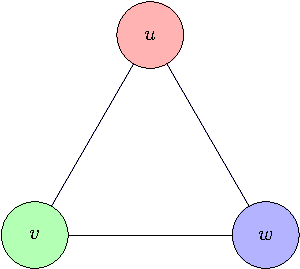
\includegraphics[height=29mm]{Resources/InsertVertexInside-Example-1.pdf}}
	\quad
	\subfigure[]{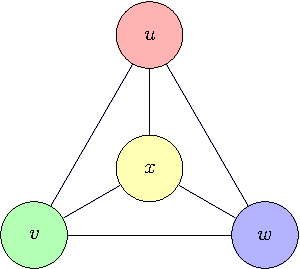
\includegraphics[height=29mm]{Resources/InsertVertexInside-Example-2.pdf}}
	\qquad
	\subfigure[]{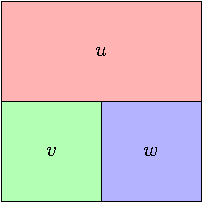
\includegraphics[height=29mm]{Resources/InsertVertexInside-Example-3.pdf}}
	\quad
	\subfigure[]{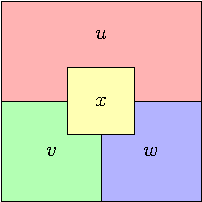
\includegraphics[height=29mm]{Resources/InsertVertexInside-Example-4.pdf}}
	\caption{A cluster graph and a polygonal dual thereof, before (a, c) and after (b, d) inserting the vertex $x$ in the triangular face $uvw$.}
	\label{fig:insert-vertex-inside-example}
\end{figure}

Let $u$, $v$, and $w$ be the vertices bounding an internal face of the cluster graph in counterclockwise order and $x$ the new vertex we want to add inside said face. We compute the paths that form the $u$-$v$-, $v$-$w$-, and $w$-$u$-boundaries in the polygonal dual. Let $p_{uvw}$ denote the vertex where the three faces corresponding to $u$, $v$, and $w$ meet. Let $p_{uv}$, $p_{vw}$, and $p_{wu}$ denote the first subdivision vertex on the boundary between faces $u$ and $v$, $v$ and $w$, and $w$ and $u$, respectively, starting from $p_{uwv}$. If one of the boundaries consist of only one edge, we place a subdivision vertex at its midpoint first. \Cref{subfig:insert-vertex-inside-illustration-1} shows how these vertices might look for the example from above.

\begin{figure}[H]
	\centering
	\subfigure[]{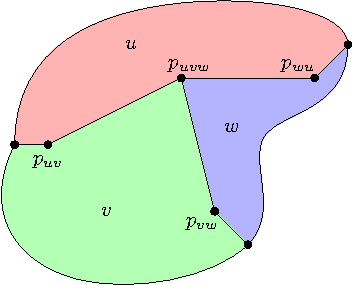
\includegraphics[width=45mm]{Resources/InsertVertexInside-Illustration-1.pdf}\label{subfig:insert-vertex-inside-illustration-1}}
	\quad
	\subfigure[]{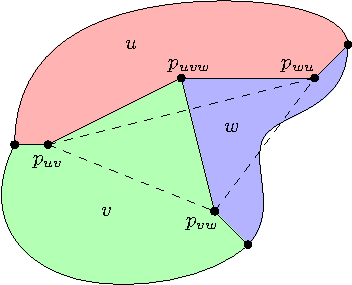
\includegraphics[width=45mm]{Resources/InsertVertexInside-Illustration-2.pdf}\label{subfig:insert-vertex-inside-illustration-2}}
	\quad
	\subfigure[]{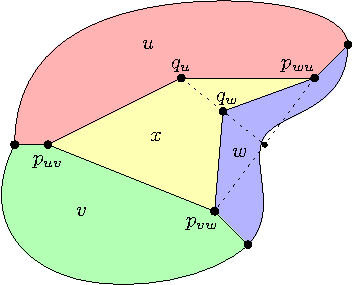
\includegraphics[width=45mm]{Resources/InsertVertexInside-Illustration-3.pdf}\label{subfig:insert-vertex-inside-illustration-3}}
	\caption{Inserting an internal face $x$ at the point where three faces $u,v,w$ meet.}
	\label{fig:insert-vertex-inside-illustration}
\end{figure}

Having determined the subdivision vertices $p_{uv}$, $p_{vw}$, and $p_{wu}$, we now want to remove the vertex $p_{uvw}$ and insert edges between the subdivision vertices instead to bound a new face for $d$ (dashed lines in \cref{subfig:insert-vertex-inside-illustration-2}). Doing so naïvely may introduce edge crossings and we generally need to add bends in the form of subdivision vertices to those edges. We distinguish three cases, all of which are illustrated in the figure:
%
\begin{itemize}
	\item If we can place an edge between $p_{ab}$ and $p_{bc}$ without introducing an edge crossing, we do not need to bend the edge (face $v$ in \cref{subfig:insert-vertex-inside-illustration-3}).
	\item Otherwise, if the internal angle of face $a$ at $p_{abc}$ is more than half a turn, we place the bend $q_a$ at $p_{abc}$ (face $u$ in \cref{subfig:insert-vertex-inside-illustration-3}).
	\item Otherwise we search for a bend location $q_a$ somewhere on the line segment from the midpoint of $p_{ab}$ and $p_{bc}$ to $p_{abc}$. We start at the midpoint of $p_{ab}$ and $p_{bc}$ and divide the remaining distance to $p_{abc}$ in half until we find a bend location for which the bent edge from $p_{ab}$ to $p_{bc}$ would not create edge crossings (face $w$ in \cref{subfig:insert-vertex-inside-illustration-3}).
\end{itemize}

Considering at most one angle at $p_{uvw}$ can be more than half a turn, we place at most one bend there. By removing the vertex $p_{uvw}$ and inserting the edges $\{p_{uv},p_{vw}\}$, $\{p_{vw},p_{wu}\}$, and $\{p_{wu},p_{uv}\}$, potentially with bends $p_v$, $p_w$, and $p_u$, we create an internal face for $x$.



\paragraph{Inserting Vertices Outside}

Alternatively, we can add a new vertex in the outer face of the cluster graph. Such a vertex must be connected to at least two vertices on the outer face to preserve the graph's 2-connectivity and its neighbors must form a path on the original boundary of the cluster graph in order not to create holes and thereby violate its internal triangulatedness.

We restrict ourselves to adding new vertices in the outer face that are made incident to exactly 2 neighboring vertices. Let $\{u,v\}$ be an edge on the outer face, then we support adding a new vertex $x$ in the outer face and connecting it to both $u$ and $v$. \Cref{fig:insert-vertex-outside-example} illustrates a valid vertex insertion into the outer face.

\begin{figure}[H]
	\centering
	\subfigure[]{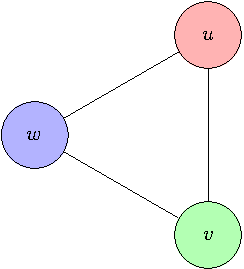
\includegraphics[height=29mm]{Resources/InsertVertexOutside-Example-1.pdf}}
	\quad
	\subfigure[]{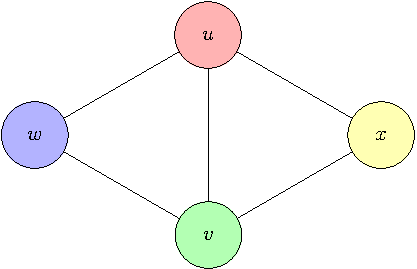
\includegraphics[height=29mm]{Resources/InsertVertexOutside-Example-2.pdf}}
	\qquad
	\subfigure[]{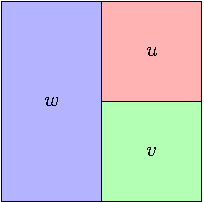
\includegraphics[height=29mm]{Resources/InsertVertexOutside-Example-3.pdf}}
	\quad
	\subfigure[]{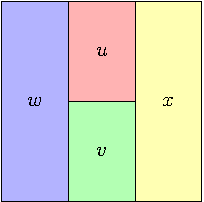
\includegraphics[height=29mm]{Resources/InsertVertexOutside-Example-4.pdf}}
	\caption{A cluster graph and a polygonal dual thereof, before (a, c) and after (b, d) inserting the vertex $x$ on the outer face and connecting it to $u$ and $v$.}
	\label{fig:insert-vertex-outside-example}
\end{figure}

Let $u$ and $v$ be the adjacent vertices on the outer face of the cluster graph and $x$ the new vertex we want to add in the outer face.
Let $p_{uv}$ denote the vertex where the faces $u$ and $v$ meet the outer face of the polygonal dual.
We define $p_u$ and $p_v$ as the first subdivision vertex we encounter when starting at $p_{uv}$ and following the boundary of $u$ and $v$ with the outer face, respectively.
If one of the boundaries consist of only one edge, we place a subdivision vertex at its midpoint and use that vertex as $p_u$/$p_v$.
\Cref{subfig:insert-vertex-outside-illustration-1} shows how these vertices might look for the example from above.
%

\begin{figure}[H]
	\centering
	\subfigure[]{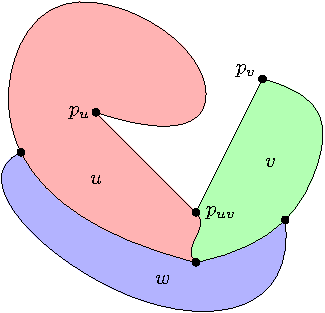
\includegraphics[width=45mm]{Resources/InsertVertexOutside-Illustration-1.pdf}\label{subfig:insert-vertex-outside-illustration-1}}
	\quad
	\subfigure[]{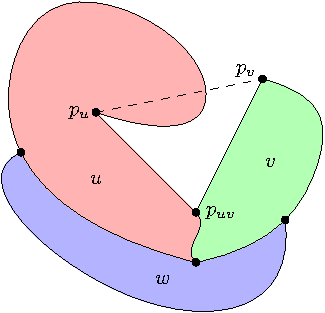
\includegraphics[width=45mm]{Resources/InsertVertexOutside-Illustration-2.pdf}\label{subfig:insert-vertex-outside-illustration-2}}
	\quad
	\subfigure[]{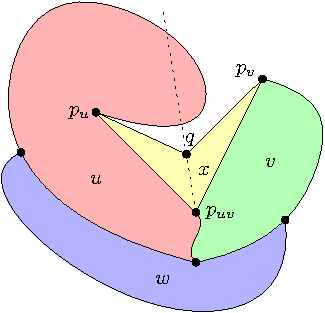
\includegraphics[width=45mm]{Resources/InsertVertexOutside-Illustration-3.pdf}\label{subfig:insert-vertex-outside-illustration-3}}
	\caption{Inserting a face $x$ at the point where the faces $u$ and $v$ meet the outer face.}
	\label{fig:insert-vertex-outside-illustration}
\end{figure}

With $p_u$ and $p_v$ determined, we can create the face $x$ by inserting a path to connect $p_u$ and $p_v$ without introducing edge crossings. Simply inserting an edge between $p_u$ and $p_v$ generally isn't enough, as illustrated in \cref{subfig:insert-vertex-outside-illustration-2}. However, with a single bend in the form of a subdivision vertex $q$, we can guarantee that no edge crossings are being created.

We search for a bend location on the outward-pointing bisector of the angle $\measuredangle_{p_up_{uv}p_v}$, starting at some fixed distance $\epsilon > 0$ and halving the distance until we find a valid location. As the possible bend location moves infinitesimally close to $p_{uv}$, we are guaranteed to find one that doesn't introduce edge crossings. By inserting a vertex at $q$ along with edges $\{q,p_u\}$ and $\{q,p_v\}$, we create an internal face for $x$, as illustrated in \cref{subfig:insert-vertex-outside-illustration-3}.

\clearpage
\section{Removing Vertices}
\label{sect:removing-vertices}

Clusters in the underlying data set can also fade and eventually cease to exist. In this case, we want to be able to remove existing vertices of the cluster graph. We make the same distinction here as when inserting vertices: we can remove internal vertices or vertices that lie on the cluster graph's outer face. 



\paragraph{Removing Internal Vertices}

When removing an internal vertex, we must ensure that the cluster graph remains internally triangulated. This is only the case if the vertex we want to remove has degree 3 as removing vertices with greater degree would create holes. If one wants to a vertex with degree 4 or higher, one must first tweak the adjacencies on the inside of the cluster graph using edge flips, discussed in \cref{sect:flipping-edges}. \Cref{fig:remove-vertex-example-internal} shows a valid removal of an internal vertex.

\begin{figure}[H]
	\centering
	\subfigure[]{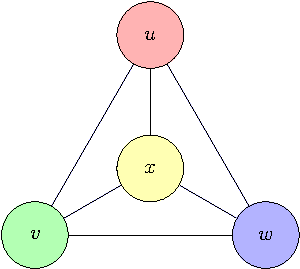
\includegraphics[height=29mm]{Resources/RemoveVertex-Example-Internal-1.pdf}}
	\quad
	\subfigure[]{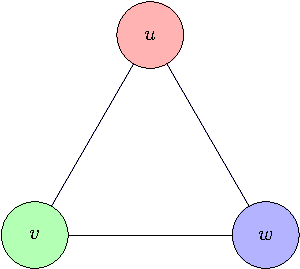
\includegraphics[height=29mm]{Resources/RemoveVertex-Example-Internal-2.pdf}}
	\qquad
	\subfigure[]{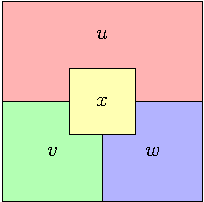
\includegraphics[height=29mm]{Resources/RemoveVertex-Example-Internal-3.pdf}}
	\quad
	\subfigure[]{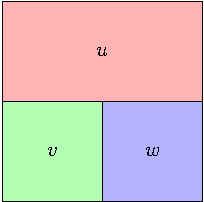
\includegraphics[height=29mm]{Resources/RemoveVertex-Example-Internal-4.pdf}}
	\caption{A cluster graph and a polygonal dual thereof, before (a, c) and after (d, d) removing the internal vertex $x$ with degree 3.}
	\label{fig:remove-vertex-example-internal}
\end{figure}

In order not to create holes in the contact representation, the incident faces must take over the area that the face to be removed originally occupied. Let $x$ denote the internal vertex we want to remove and $u$, $v$, and $w$ its three neighbors. We start by computing the paths that form the $u$-$v$-, $v$-$w$, and $w$-$u$-boundaries in the dual. Let $p_{uvx}$ ($p_{vwx}$, $p_{uwx}$) denote the vertex where face $x$ meets faces $u$ and $v$ ($v$ and $w$, $w$ and $u$). \Cref{subfig:remove-vertex-illustration-1} shows how these vertices might look for the example from above.

\begin{figure}[H]
	\centering
	\subfigure[]{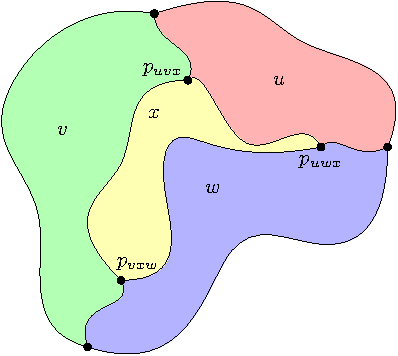
\includegraphics[width=45mm]{Resources/RemoveVertex-Illustration-1.pdf}\label{subfig:remove-vertex-illustration-1}}
	\quad
	\subfigure[]{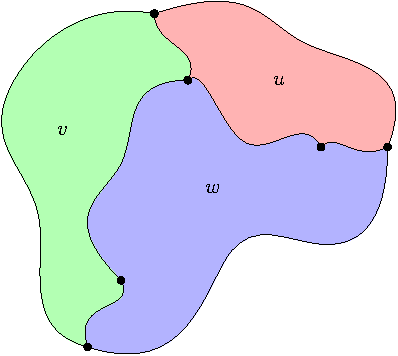
\includegraphics[width=45mm]{Resources/RemoveVertex-Illustration-2.pdf}\label{subfig:remove-vertex-illustration-2}}
	\caption{Removing an internal face $x$ incident to the faces $u$, $v$, and $w$.}
	\label{fig:remove-vertex-illustration}
\end{figure}

To remove the internal face $x$, we simply remove the its boundary to one of its neighboring faces. In doing so, the two faces effectively merge. In practice this works really well because large clusters don't disappear at a moment's notice, and small clusters generally occupy a very small area such that the operation is barely noticeable.




\paragraph{Removing External Vertices}

When removing vertices on the outer face along with its incident edges, we must ensure that the graph remains 2-connected afterwards. \cref{fig:remove-vertex-example-external} illustrates a valid removal of a vertex on the outer face. Similar to inserting vertices on the outer face, we restrict ourselves to removing vertices on the outer face that have degree 2. If we need to remove a vertex with higher degree, the additional edges need to be removed first as discussed in \cref{sect:flipping-edges}.

\begin{figure}[H]
	\centering
	\subfigure[]{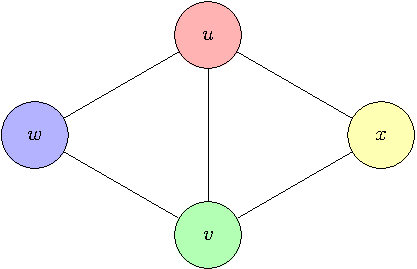
\includegraphics[height=29mm]{Resources/RemoveVertex-Example-External-1.pdf}}
	\quad
	\subfigure[]{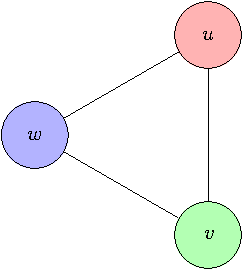
\includegraphics[height=29mm]{Resources/RemoveVertex-Example-External-2.pdf}}
	\qquad
	\subfigure[]{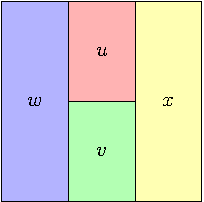
\includegraphics[height=29mm]{Resources/RemoveVertex-Example-External-3.pdf}}
	\quad
	\subfigure[]{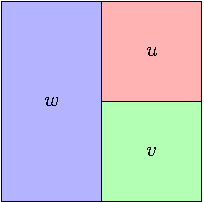
\includegraphics[height=29mm]{Resources/RemoveVertex-Example-External-4.pdf}}
	\caption{A cluster graph and a polygonal dual thereof, before (a, c) and after (b, d) removing the vertex $x$ on the outer face.}
	\label{fig:remove-vertex-example-external}
\end{figure}

This operation, too, is just a special case of the vertex removal discussed above. Referring to the construction of the augmented dual again, with the helper vertex $v^+$ and edges $\{v^+,\cdot\}$, removable vertices $x$ on the outer face of the cluster graph lie in a triangle formed by its two neighbors $u$ and $v$ and the helper vertex $v^+$.

The construction outlined above translates 1-to-1 to removing vertices from the outer face, except one of the three neighboring faces is the implicit outer face. In our implementation, we always remove the boundary of $x$ with the outer face and thereby transfer the area to the outer face.

\clearpage
\section{Flipping Edges}
\label{sect:flipping-edges}

Let us now discuss the edge flip mentioned in the previous sections.
An internal edge $\{u,v\}$ is incident to two different internal faces $f$, $g$.
Let $x$ and $y$ denote the third vertex bounding $f$ and $g$, respectively.
It is $x \neq y$ because the cluster graph is simple.
Flipping the edge $\{u,v\}$ would replace it with the edge $\{x,y\}$.
Consequently, this operation is only permitted iff $x$ and $y$ are not already adjacent \emdash{} otherwise, we would introduce a duplicate adjacency.
\Cref{fig:flip-edge-example-internal} shows an example of a valid edge flip operation.

\begin{figure}[H]
	\centering
	\subfigure[]{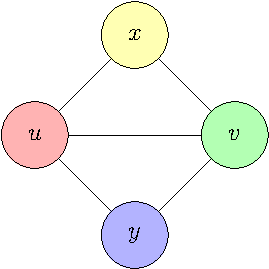
\includegraphics[height=28mm]{Resources/FlipEdge-Example-Internal-1.pdf}}
	\quad
	\subfigure[]{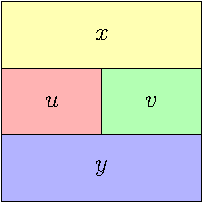
\includegraphics[height=28mm]{Resources/FlipEdge-Example-Internal-2.pdf}}
	\qquad
	\subfigure[]{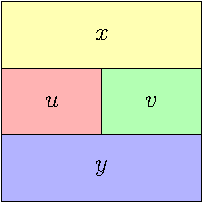
\includegraphics[height=28mm]{Resources/FlipEdge-Example-Internal-3.pdf}}
	\quad
	\subfigure[]{\includegraphics[height=28mm]{Resources/FlipEdge-Example-Internal-4.pdf}}
	\caption{A cluster graph and a polygonal dual thereof, before (a, c) and after (b, d) flipping the internal edge $\{u,v\}$.}
	\label{fig:flip-edge-example-internal}
\end{figure}

An edge flip in a cluster graph translates to region adjacencies being flipped in its dual.
Given a polygonal dual of some cluster graph, we apply an edge flip in two phases.
First, we contract the region boundary we want to remove into a single point, creating a degenerate contact representation in which four regions meet in a point.
In the second phase, we create a region boundary in the opposite direction, getting rid of the degeneracy at the point into which the original boundary has been contracted.

Let $u$ and $v$ be two adjacent faces in the polygonal dual whose boundary we want to contract.
Also, let path $P_{uv}$ be the maximal common boundary between $u$ and $v$, oriented such that $u$ lies on the left of it, and $v$ lies on the right of it.
At both endpoints of the path, $u$ and $v$ meet with a third face.
We denote the third face incident to the path's first vertex by $x$ and the third face incident to the path's last vertex by $y$, as illustrated in \cref{fig:flip-edge-example-internal}.
To contract the $u$-$v$-boundary into a single point, we repeatedly contract a peripheral edge on the boundary until the last edge has been contracted.
We do so on alternating ends, \ie{}, we start by contracting the first edge, then the last, then the first again, etc.

\begin{figure}[H]
	\centering
	\subfigure[]{\includegraphics[width=40mm]{Resources/FlipEdge-ContractBoundaryBelow-1.pdf}\label{subfig:flip-edge-contract-boundary-below-1}}
	\quad
	\subfigure[]{\includegraphics[width=40mm]{Resources/FlipEdge-ContractBoundaryBelow-2.pdf}\label{subfig:flip-edge-contract-boundary-below-2}}
	\quad
	\subfigure[]{\includegraphics[width=40mm]{Resources/FlipEdge-ContractBoundaryBelow-3.pdf}\label{subfig:flip-edge-contract-boundary-below-3}}
	\caption{A contact representation before (a) and after (c) contracting the peripheral edge $\{p_{uv},p_{uvy}\}$ on the $u$-$v$-boundary away from $y$. (b) shows the construction of potential subdivision vertices.}
	\label{fig:flip-edge-contract-boundary-below}
\end{figure}

\Cref{fig:flip-edge-contract-boundary-below} illustrates how we contract the first edge of the oriented upwards without introducing edge crossings.
We describe only this construction in writing; the contraction of the last edge works virtually the same way and is illustrated in \cref{fig:flip-edge-contract-boundary-above}.
Let $p_{uvy}$ denote the vertex where the faces $u$, $v$, and $y$ meet and $p_{uy}$ and $p_{vy}$ the subdivision vertices on the $u$-$y$- and $v$-$y$-boundaries that are incident to $p_{uvy}$, respectively.
If the $u$-$y$- or $v$-$y$-boundary consists of only one edge, we subdivide it at its midpoint first.
Let $p_{uv}$ be the subdivision vertex on the $u$-$v$-boundary that is incident to $p_{uvy}$ or the last vertex of the oriented boundary if no such subdivision vertex exists.
To reduce the length of the $u$-$v$-boundary by one, we would want to remove $p_{uvy}$ and its incident edges and add edges from $p_{uv}$ to both $p_{uy}$ and $p_{vy}$.
These edges may introduce crossings, though, as illustrated by the dashed lines in \cref{subfig:flip-edge-contract-boundary-above-2} and \cref{subfig:flip-edge-contract-boundary-below-2}.
However, with just one bend on each of the edges, we can guarantee that no edge crossings are created:

\begin{itemize}
\item If adding the edge between $p_{uv}$ and $p_{ay}$ ($a \in \{u,v\}$) does not introduce a crossing, we simply add the edge.
(for $a = u$ in \cref{subfig:flip-edge-contract-boundary-below-2})
\item Otherwise, if the internal angle of face $a$ at $p_{uvy}$ is $180^\circ$ or more, we place the bend at $p_{uvy}$, \ie{}, we insert the edge $\{p_{uv},p_{ay}\}$ and subdivide it with a new vertex $q_{ay}$ at the position of $p_{uvy}$.
Note that at most one of the faces can have an internal angle at $p_{uvy}$ that is $180^\circ$ or more.
(for $a = v$ in \cref{subfig:flip-edge-contract-boundary-above-2})
\item Otherwise, we search for a bend location in the form of a subdivision vertex $q_{ay}$ somewhere on the outward-pointing bisector of the angle $\angle_{p_{ay}p_{uvy}p_{uv}}$ (dotted lines in \cref{subfig:flip-edge-contract-boundary-below-2} and \cref{subfig:flip-edge-contract-boundary-above-2}).
We start looking at the point where the bisector intersects the segment from $p_{uv}$ to $p_{ay}$ and repeatedly divide the remaining distance to $p_{uvy}$ in half until we find a bend location for which the bent edge from $p_{uv}$ to $p_{ay}$ would not introduce edge crossings.
As the candidate location moves infinitesimally close to $p_{uvy}$, we are guaranteed to find one that does not introduce crossings.
(for $a = v$ in \cref{subfig:flip-edge-contract-boundary-below-3} and $a = u$ in \cref{subfig:flip-edge-contract-boundary-above-3})
\end{itemize}

\begin{figure}[H]
	\centering
	\subfigure[]{\includegraphics[width=40mm]{Resources/FlipEdge-ContractBoundaryAbove-1.pdf}\label{subfig:flip-edge-contract-boundary-above-1}}
	\quad
	\subfigure[]{\includegraphics[width=40mm]{Resources/FlipEdge-ContractBoundaryAbove-2.pdf}\label{subfig:flip-edge-contract-boundary-above-2}}
	\quad
	\subfigure[]{\includegraphics[width=40mm]{Resources/FlipEdge-ContractBoundaryAbove-3.pdf}\label{subfig:flip-edge-contract-boundary-above-3}}
	\caption{A contact representation before (a) and after (c) contracting the last remaining edge $\{p_{uvx},p_{uvy}\}$ on the $u$-$v$-boundary away from $y$. (b) shows the construction of potential subdivision vertices.}
	\label{fig:flip-edge-contract-boundary-above}
\end{figure}

Once the $u$-$v$-boundary has been contracted into a single vertex $p_{uvxy}$ where all four faces $u$, $v$, $x$, and $y$ now meet, as shown in \cref{subfig:flip-edge-contract-boundary-above-3}, we need to resolve the degeneracy and create a boundary in the opposite direction, \ie{}, an $x$-$y$-boundary.
Let $p_{ux}$, $p_{uy}$, $p_{vx}$, and $p_{vy}$ denote the subdivision vertices on the respective boundaries that are incident to $p_{uvxy}$.
Again, if a boundary consists of only one edge, we subdivide it at its midpoint first such that all $p_{ab}$ exist.
We are now looking to stretch the vertex $p_{uvxy}$ back into a non-degenerate $x$-$y$-boundary, as illustrated in \cref{fig:flip-edge-create-boundary}.
Analogous to above, we search for a position in face $u$ ($v$) where we can place a vertex $q_u$ ($q_v$) and add edges to $p_{uvxy}$, $p_{ux}$, and $p_{uy}$ ($p_{uvxy}$, $p_{vx}$, and $p_{vy}$) without introducing crossings.
We start at the intersection of the segment between $p_{ux}$ and $p_{uy}$ (between $p_{vx}$ and $p_{vy}$) and the bisector of $\angle_{p_{ux}p_{uvxy}p_{uy}}$ ($\angle_{p_{vx}p_{uvxy}p_{vy}}$) and repeatedly divide the distance to $p_{uvxy}$ in half until we find a valid position.
Once we have found such a position, we insert the vertex $q_u$ ($q_v$) along with the aforementioned edges and remove the edges $\{p_{uvxy},p_{ux}\}$ and $\{p_{uvxy},p_{uy}\}$ ($\{p_{uvxy},p_{vx}\}$ and $\{p_{uvxy},p_{vy}\}$).
In case $\measuredangle_{p_{ux}p_{uvxy}p_{uy}} \geq 180^\circ$ ($\measuredangle_{p_{vx}p_{uvxy}p_{vy}} \geq 180^\circ$), we will not find such a position and shall not make an adjustment on that side.
However, again, this event cannot occur for both $u$ and $v$ at the same time.
As a result, we always create an $x$-$y$-boundary that consists of at least one edge.

\begin{figure}[H]
	\centering
	\subfigure[]{\includegraphics[width=45mm]{Resources/FlipEdge-StretchBoundary-1.pdf}}
	\quad
	\subfigure[]{\includegraphics[width=45mm]{Resources/FlipEdge-StretchBoundary-2.pdf}}
	\quad
	\subfigure[]{\includegraphics[width=45mm]{Resources/FlipEdge-StretchBoundary-3.pdf}}
	\caption{A contact representation before (a) and after (c) creating a non-degenerate yellow-blue adjacency. (b) shows the construction of potential subdivision vertices.}
	\label{fig:flip-edge-create-boundary}
\end{figure}



\paragraph{Inserting and Removing Edges}

As clusters in our data set grow increasingly similar, we may want to indicate this similarity with new edges between existing clusters in the cluster graph.
Similarly, clusters can grow apart, and we may want to remove edges between clusters in the cluster graph.
However, because the filtered cluster graph is internally triangulated, we cannot insert any more edges on the inside of the graph.
Removing an internal edge is not permitted either, as that would create a hole in the graph.
Consequently, we can insert edges only in the outer face and remove edges only on the outer face.

On top of that, inserting an edge in the outer face is only possible if it preserves the cluster graph's internal triangulatedness.
Therefore, inserting an edge $\{u,w\}$ is only permitted iff $u$ and $w$ lie on the outer face and have a neighbor $v$ in common that also lies on the outer face.
The inserted edge is then embedded such that it forms a new triangular internal face with $v$ and turns $v$ into an internal vertex.
If exactly four vertices bound the outer face before inserting the edge $\{u,w\}$, there exist two candidates for $v$.
In this case, it must be made explicit which one is supposed to become internal and which one is supposed to remain on the outer face.
\Cref{fig:flip-edge-example-insert} shows an example of a valid edge insertion.

\begin{figure}[H]
	\centering
	\subfigure[]{\includegraphics[height=28mm]{Resources/FlipEdge-Example-Insert-1.pdf}}
	\quad
	\subfigure[]{\includegraphics[height=28mm]{Resources/FlipEdge-Example-Insert-2.pdf}}
	\qquad
	\subfigure[]{\includegraphics[height=28mm]{Resources/FlipEdge-Example-Insert-3.pdf}}
	\quad
	\subfigure[]{\includegraphics[height=28mm]{Resources/FlipEdge-Example-Insert-4.pdf}}
	\caption{A cluster graph and a polygonal dual thereof, before (a, c) and after (b, d) inserting the edge $\{u,w\}$ to form an internal triangular face with $v$.}
	\label{fig:flip-edge-example-insert}
\end{figure}

Removing an edge $\{u,w\}$ on the outer face of the cluster graph is only permitted if the graph remains biconnected.
This property is preserved iff both $u$ and $w$ have degree $d(\cdot) \geq 3$ and the third vertex $v$ in the internal face bounded by $\{u,w\}$ does not already lie on the outer face.
If that vertex laid on the outer face already, we would end up creating a duplicate adjacency/boundary between $v$ and the outer face, which we specifically excluded in \cref{chap:preliminaries}.
\Cref{fig:flip-edge-example-remove} shows an example of a valid edge removal.

\begin{figure}[H]
	\centering
	\subfigure[]{\includegraphics[height=28mm]{Resources/FlipEdge-Example-Remove-1.pdf}}
	\quad
	\subfigure[]{\includegraphics[height=28mm]{Resources/FlipEdge-Example-Remove-2.pdf}}
	\qquad
	\subfigure[]{\includegraphics[height=28mm]{Resources/FlipEdge-Example-Remove-3.pdf}}
	\quad
	\subfigure[]{\includegraphics[height=28mm]{Resources/FlipEdge-Example-Remove-4.pdf}}
	\caption{A cluster graph and a polygonal dual thereof, before (a, c) and after (b, d) removing the edge $\{u,w\}$.}
	\label{fig:flip-edge-example-remove}
\end{figure}

Both of these operations are again a special case of the generic edge flip discussed above with a quirk:
Instead of four internal faces, they involve three internal faces and the implicit outer face.

In the example from \cref{fig:flip-edge-example-insert}, we make $v$ into an internal vertex by inserting the edge $\{u,w\}$, removing $v$'s boundary with the outer face in the dual and creating a $u$-$w$-boundary in turn.
Again, recall that in the construction of the augmented dual from \cref{def:augmented-dual}, we insert a helper vertex $v^+$ in the outer face and add edges to all vertices on the original outer face.
This helper vertex and its adjacencies correspond to the outer face and its boundaries in the dual.
When inserting an edge in the outer face, we are essentially flipping the helper edge $\{v,v^+\}$ to become the inserted edge $\{u,w\}$.
Therefore, we apply the same procedure as discussed for the edge flip above, contracting the boundary between $v$ and the outer face into a single point and then creating a non-degenerate $u$-$w$-boundary.

Similarly, when removing an edge $\{u,w\}$ on the outer face as in \cref{fig:flip-edge-example-remove}, a previously-internal vertex $v$ moves onto the outer face.
We can think of it as flipping the edge to be removed to become the helper edge $\{v,v^+\}$.
In the polygonal dual, this gets rid of the $u$-$w$-boundary and creates a boundary between $v$ and the implicit outer face in turn.
Again, we apply the same procedure as discussed for the edge flip, first contracting the $u$-$w$-boundary into a single point and then creating a non-degenerate boundary between $v$ and the outer face.


\chapter{Experimental Evaluation}
\label{chap:experimental-evaluation}

In this chapter, we experimentally evaluate the our implementation of the framework discussed in \crefrange{chap:visualizing-static-input-graphs}{chap:visualizing-dynamic-input-graphs} in order to gain insights into areas that may need to be improved upon in future research.
As part of our evaluation, we give answers to the following research questions:

\begin{enumerate}
	\item Which quality metrics best capture the accuracy of the maps generated by our algorithm in terms of
	\begin{enumerate}
	\item accuracy?
	\item our understanding of locally fat regions?
	\end{enumerate}
	\item What is the quality of the maps generated by our algorithm according to these quality metrics?
	\begin{enumerate}
	\item How does this quality change based on the size of the input graph?
	\item How does this quality change over time as dynamic updates are incorporated?
	\end{enumerate}
\end{enumerate}

First, we discuss a variety of possible quality metrics from literature and how they can be applied to our framework in \cref{sect:quality-metrics}.
We pick two metrics to proceed with that best capture the quality of the generated maps according to research question 1.
In \cref{sect:test-case-generation} we present the algorithm we use to generate randomized test instances to perform our experimental evaluation with.
Eventually, in \cref{sect:evaluation}, we conduct the actual evaluation on a large number of test instances and see how the maps generated by our algorithm perform, thereby answering research question 2.

\section{Quality Metrics}
\label{sect:quality-metrics}

We start by looking at common quality metrics of cartograms, which are closely related to the problem we are trying to solve in this thesis as previously discussed in \cref{sect:related-work}, and discussing how they translate to the visualizations our framework creates.
We then discuss different ideas to formalize and quantify the previously mentioned notion of local fatness of the regions.



\paragraph{Quality Metrics of Cartograms}

Three well-established quantifiable measures are commonly used to assess a cartograms's quality \cite{alam2015quantitative} \cite{nusrat2018evaluating}:

\begin{itemize}
\item \textbf{Statistical accuracy:}
The statistical accuracy of a cartogram describes how closely the areas of the modified geographic regions match the variable of interest.
Recall that the normalized cartographic error of a region $v$ is defined as $\frac{\abs{A^\prime(v)-w(v)}}{max(A^\prime(v),w(v))}$ where $A^\prime(v)$ is its normalized actual area and $w(v)$ is its desired area.
The maximum and average normalized cartographic error over all regions in the cartogram are commonly used to quantify its statistical accuracy.
We borrow this quality metric from cartograms as we have already used it previously to define $\varepsilon$-proportional maps.

\item \textbf{Topological accuracy:}
The topological accuracy describes how well the original adjacencies between the geographic regions are preserved in the cartogram.
Considering our framework computes a polygonal contact representation of the filtered cluster graph, those and only those regions whose corresponding vertices are adjacent in the cluster graph are adjacent in the contact representation.
In terms of topological accuracy, we therefore produce perfect drawings.

\item \textbf{Geographic accuracy:}
The geographic accuracy of a cartogram describes to what degree the shapes and positions of the distorted regions resemble their original counterpart on the real geographic map.
In our case, however, there is no real geographic map that our visualization is based upon:
The maps we generate are entirely artificial and there is no geographic reference map.

However, the motivation behind geographic accuracy as a quality metric still makes sense in our setting.
Geographic accuracy captures the preservation of the viewer's mental map between the real geographic map and the distorted map in the cartogram.
And this applies to our framework as well, albeit only once we start incorporating dynamic updates into the artificial map.
Our dynamic pipeline naturally preserves the viewer's mental map by only allowing small, incremental changes to be incorporated and redrawing the artificial map using a force-directed algorithm.
This makes it easy for the viewer to track how the map changes between versions of the underlying cluster graph at different points in time.
\end{itemize}



\paragraph{Polygon Complexity}

Brinkhoff \etal{} \cite{brinkhoff1995measuring} propose a method to quantify the complexity of polygons.
They measure the complexity of polygons as a combination of three properties: the frequency of the vibration of its boundary, the amplitude of said vibration, and the deviation from its convex hull.
Given a polygon $P$, they count the number of corners where the polygon's internal angle is more than $180^\circ$, called \emph{notches}, and define the fraction of those corners as
%
\begin{equation*}
\text{notches}_{\lbrack0,1\rbrack}(P) \coloneqq
\begin{cases}
\frac{\text{notches}(P)}{n - 3} & \text{if $n$ > 3}\\
0 & \text{otherwise}
\end{cases}
\in \lbrack0,1\rbrack
,
\end{equation*}
%
where $n$ is the total number of corners in $P$ and $\text{notches}(P)$ the number of corners that are notches.
They use this fraction to define the frequency of the vibration as
%
\begin{equation*}
\text{freq}(P) \coloneqq 1
+ 16 \cdot (\text{notches}_{\lbrack0,1\rbrack}(P) - 0.5)^4
- 8 \cdot (\text{notches}_{\lbrack0,1\rbrack}(P) - 0.5)^2
\in \lbrack0,1\rbrack
\end{equation*}
%
and its amplitude as
\begin{equation*}
\text{ampl}(P) \coloneqq
\frac{\text{circumference}(P) - \text{circumference}(\text{hull}(P))}{\text{circumference}(P)}
\in \lbrack0,1\rbrack
,
\end{equation*}
%
where $\text{circumference}(P)$ is the the length of $P$'s boundary and $\text{hull}(P)$ is the convex hull of $P$'s corners in the form of another polygon.
These equations were chose such that the frequency $\text{freq}(P)$ of the vibration of a polygon reaches its maximum when half of the polygon's corners are notches, and the amplitude $\text{ampl}(P)$ of the vibration is close to 1 when the area of the polygon is very small in relation to the area of it's convex hull.
Intuitively, for convex polygons $P$, both the frequency $\text{freq}(P)$ and the amplitude $\text{ampl}(P)$ of the vibration of its boundary is zero.

To measure the convexity of a polygon, Brinkhoff \etal{} use the fraction of the area of the polygon's convex hull that the polygon itself covers:
%
\begin{equation*}
\text{conv}(P) \coloneqq
\frac{\text{area}(\text{hull}(P)) - \text{area}(P)}{\text{area}(\text{hull}(P))}
\in \lbrack0,1\rbrack
\end{equation*}

According to their observations, a relative increase of the boundary in combination with a high-frequency vibration of the boundary has the most significant impact on the intuitive perception a polygon's complexity \cite{brinkhoff1995measuring}.
They therefore combine these three properties as
%
\begin{equation}
\text{compl}(P) \coloneqq
0.8 \cdot \text{ampl}(P) \cdot \text{freq}(P) + 0.2 \cdot \text{conv}(P)
\in \lbrack0,1\rbrack
\end{equation}
%
to measure the overall complexity of a polygon.

We adopt this definition of polygon complexity as a quality metric for the maps generated by our framework, but only with a slight change because as is, $\text{compl}(\cdot)$ assigns a perfect score of $0$ to all convex polygons.
This means that, for example, there is no distinction between a square region and a long, drawn-out rectangular region, even though the square regions matches our understanding of local fatness much better.
Instead of calculating the fraction of area a polygon $P$ doesn't cover within its convex hull, we therefore compute the fraction of area it doesn't cover in its smallest enclosing circle.
To keep $\text{conv}(\cdot)$ in unit interval, we actually compare $P$'s area to the maximal area of a regular $n$-gon in said smallest enclosing circle:
%
\begin{equation*}
\text{compl}^\prime(P) \coloneqq
1 - \frac{\text{area}(P)}{\text{area}(\text{smallestEnclosingCircle}(P)) \cdot \sin\left(\frac{360^\circ}{n}\right) \cdot \frac{n}{2\pi}}
\in \lbrack0,1\rbrack
\end{equation*}

In our tests, this measure has shown to align with our intuitive understanding of local fatness nicely.



\paragraph{Entropy}

Chen and Sundaram \cite{chen2005estimating} studied the complexity of 2-dimensional shapes in the field of computer vision.
The shapes they dealt with are given in the form of a point cloud.
For each point, they compute the Euclidean distance to the point cloud's centroid.
They also implement a heuristic to predict the contour of the shape at each point and use it to compute a local angle for each of the points.
The distances and local angles are then plotted into a histogram with flexible bin size and are used to compute the entropy of the distribution of distances and local angles.

In our use case, we don't even have to implement the heuristic to guess the shape's contour.
We know that the points form a closed curve that is in fact a polygon.
However, by connecting the points in this predetermined manner, we possibly get drastically different edge lengths.
The points on these edges that aren't corners of the polygon have no impact on the computed entropies at all.
This problem becomes obvious when we consider two straight-line segments of the same length, one that is a single side of our polygon, and one which is the union of multiple sides of our polygon with corners (with internal angle $180^\circ$) in between:
The one with additional corners has a much greater impact on the computed entropies, even though both look the same to an observer.

We can try to remedy by subdividing the polygon's sides first, creating roughly uniform side lengths.
However, in doing so, we create lots of corners at which the polygon has an internal angle of $180^\circ$, quickly dominating and distorting the entropy of internal angles.

In our tests, neither of two entropy-based measures, with or without our adjustments, captured our intuitive understanding of local fatness satisfactorily.
We therefore conduct our experimental evaluation in \cref{sect:experimental-evaluation} using just cartographic error and our modified version of polygonal complexity from Brinkhoff \etal{} \cite{brinkhoff1995measuring} discussed above.
For both measures, we will look at both the maximum and average value over all regions in the map.

\clearpage
\section{Test Case Generation}
\label{sect:test-case-generation}

We implement a randomized test case generation in two phases.
First, we generate a filtered cluster graph $G^\mathcal{C}$.
We accompany this cluster graph with a planar straight-line drawing $\Gamma^\mathcal{C}$ thereof so that such a drawing doesn't need to be calculated in retrospect as previously discussed in \cref{sect:transformation-to-dual}.
Second, we generate a sequence of dynamic operations to be applied to said cluster graph.

\paragraph{Filtered Cluster Graph Generation}

Our test case generation can be configured using the following five parameters:
%
\begin{itemize}
\item \textbf{Number of clusters:} The number of clusters $n \in \mathbb{N}, n \geq 3$ determines how many vertices the generated cluster graph $G^\mathcal{C}$ has.
\item \textbf{Bounding box:} The axis-aligned bounding box $\mathcal{A} = \lbrack x_\text{min}, x_\text{max} \rbrack \times \lbrack y_\text{min}, y_\text{max} \rbrack$ determines the area in which the cluster graph's vertices can be placed.
\item \textbf{Weight distribution:} The cluster weight distribution is given as a probability mass function $\pmf \colon \mathbb{N}_+ \to \mathbb{R}_+$ and determines how the cluster weights are distributed.
\item \textbf{Nesting ratio:} The nesting ratio $\alpha \in \lbrack 0, 1 \rbrack$ determines what fraction of the $n$ vertices are nested into other triangular faces.
\item \textbf{Nesting bias:} The nesting bias $\beta \in \lbrack 0, 1 )$ determines to what degree nesting vertices into already-nested triangular faces is preferred over nesting vertices into top-level triangles.
\end{itemize}

The idea behind generating filtered cluster graphs $G^\mathcal{C}$ is as follows:
We start by placing a number of vertices randomly within the bounding box $\mathcal{A}$ and computing a triangulation of these vertices.
We then place the remaining vertices into existing triangles based on the nesting ratio $\alpha$ and bias $\beta$, inserting additional edges to those triangles' endpoints in the process.
The algorithm is illustrated in pseudocode in \cref{alg:randomized-filtered-cluster-graph-generation} on the next page.

Obviously, the generated graph is plane and internally triangulated.
Considering a point set's triangulation covers the same area as the set's convex hull, no vertex of the generated graph can appear on its outer face more than once and the graph is therefore also biconnected.

Due to the independent sampling of vertex positions in \cref{alg:randomized-filtered-cluster-graph-generation}, vertices often clump together, especially for larger test instances.
This isn't an ideal starting position for the transformation as previously discussed in \cref{sect:transformation-to-dual} because the polygonal dual contains at least twice the number of vertices, therefore clumping even more and severely restricting the involved vertices' movement.
To address this issue, we apply a force-directed \quoted{shake} to the generated straight-line drawing $\Gamma^\mathcal{C}$ of the cluster graph while preserving its edge crossing and combinatorial properties.

We do this by defining attractive forces between pairs of adjacent vertices and strong repulsive forces between non-adjacent vertices and between edges and non-incident vertices based on their distances, and again applying the rules of ImPrEd \cite{simonetto2011impred} to prevent the introduction of edge crossings.
The repulsive forces are the same as the ones defined in \cref{sect:drawing-the-dual}, although we use a higher scaling constant of $1000$ here to really prevent the vertices from clumping together.
For the attractive force between adjacent vertices, we apply the force $F_\text{att}(u,v) \coloneqq \log(d(u,v) / 100)$ to both endpoints of an edge, directed towards each other.
Here, the value of $100$ represents our ideal edge length.
This force is based on a logarithmic springs as suggested by Eades \cite{eades84heuristic}.

\vfill

\begin{algorithm}[H]
	\caption{Randomized Filtered Cluster Graph Generation}
	\label{alg:randomized-filtered-cluster-graph-generation}
	\SetArgSty{textrm}
	\vspace{5pt}
	\KwData{bounding box $\mathcal A$, weight probability mass function $\pmf(\cdot)$, count $n$, nesting ratio $\alpha$, nesting bias $\beta$}
	\KwResult{planar straight-line drawing $\Gamma^\mathcal{C}$ of a filtered cluster graph $G^\mathcal{C}$ on $n$ vertices}
	\vspace{5pt}
	create empty straight-line drawing $\Gamma^\mathcal{C}$\;
	$k \gets \min(\floor{\alpha \cdot n}, n - 3)$ \tcp{number of nested vertices}
	\BlankLine
	\tcp{sample $n - k$ pairwise distinct points $p_i \in \mathcal{A}$}
	\ForEach{index $i \in \lbrack 0, n-k ) \cap \mathbb{N}$}{
		sample random point $p_i$ within $\mathcal{A}$ (uniformly)\;
		sample random weight $w_i$ (according to $\pmf(\cdot)$)\;
		add vertex $i$ with weight $w_i$ at position $p_i$ to $\Gamma^\mathcal{C}$\;
	}
	\BlankLine
	\tcp{create edges according to Delaunay triangulation of points}
	\ForEach{triangle $\triangle_j = (u,v,w) \in$ Delaunay triangulation of points $(p_i)_i$}{
		\ForEach{$(a,b) \in \{ (u,v), (v,w), (w,u) \}$}{
			insert edge between $a$ and $b$ in $\Gamma^\mathcal{C}$ unless edge already exists\;
		}
		register triangular face $\triangle_j$ with $\text{depth}(\triangle_i) = 1$\;
	}
	\BlankLine
	\tcp{nest remaining $k$ vertices into existing triangles}
	\ForEach{index $i \in \lbrack n - k, k ) \cap \mathbb{N}$}{
		sample random triangle $\triangle_i$ (weighted by $(1 - \beta)^{-\text{depth}(\cdot)}$)\;
		sample random point $p_i$ within $\triangle_i$ (uniformly)\;
		sample random weight $w_i$ (according to $\pmf(\cdot)$)\;
		add vertex $i$ with weight $w_i$ at position $p_i$ to $\Gamma^\mathcal{C}$\;
		add edges between $i$ and all of $\triangle_i$'s endpoints to $\Gamma^\mathcal{C}$\;
		unregister triangular face $\triangle_i$\;
		register the three new triangular faces with depth $1 + \text{depth}(\triangle_i)$\;
	}
	\BlankLine
	\Return $\Gamma^\mathcal{C}$\;
\end{algorithm}



\vspace{1cm}
\paragraph{\todo{Dynamic Operation Generation}}

from set of valid dynamic operations affecting topology (all but changing weights), pick random one

do new clusters have their weights sampled according to $\pmf$?
do we allow big clusters to just disappear?

intersperse weight changes? do we sample those according to $\pmf$ or prefer close-by weights? do we apply multiple of those at once? in combination with other operation?

idea: draw a $\Delta_w$ for each country, then apply random topology-altering operation.

\clearpage
\section{Evaluation}
\label{sect:evaluation}


% https://www.scribbr.com/dissertation/write-conclusion/
\chapter{Conclusion}
\label{chap:conclusion}

% Summarize and reflect on the research
In this thesis, we explored how cluster information in graphs can be visualized naturally as countries on a map in a dynamic setting where the graph changes over time.
We proposed a framework that produces maps whose regions' sizes are approximately proportional to the respective clusters' sizes.
The framework is also able to react to dynamic changes of the input graph in a way that preserves the viewer's mental model of the map.

% Show what new knowledge you have contributed
We are able to make these guarantees by working on an intermediate representation that encompasses all combinatorial properties of the eventual map, breaking changes down into small, incremental changes, and using a force-directed algorithm to draw the eventual map.
This way, the structure of our algorithmic pipeline alone guarantees that changes to the map are minor and comprehensible, thereby preserving the viewer's mental map as the underlying data changes over time.

Besides the preservation of the mental map, related work struggles with keeping clusters as continuous regions in the generated maps \cite{gansner2009gmap} \cite{mashima2011visualizing}.
The structure of our algorithmic pipeline addresses and solves this problem, too.
Considering the maps we produce are contact representations of the intermediate cluster graph, clusters cannot possibly be fragmented across different regions.

The framework presented here can be applied to a variety of real-world applications, allowing us to visualize clusters in the underlying data and how they change over time, thereby enabling viewers of the visualization to easily detect trends in the data.

% Clearly state the answer to the main research question

% Make recommendations for future work on the topic
\section{Future Work}
\label{sect:future-work}

There are a number of aspects of the framework discussed here that can be improved upon in future research.


\paragraph{Requirements}

First and foremost, one might relax the requirements imposed on the filtered cluster graph and adjust the implementations of the different phases of the pipeline accordingly.
For example, one could support connected but not necessarily biconnected cluster graphs.
This would allow for additional features found on many real-world geographic maps, such as regions that are adjacent to only one internal face (\eg{} Portugal) or regions that have multiple boundaries with the implicit outer face (\eg{} Spain).
Similarly, one could allow cluster graphs that aren't internally triangulated, allowing for maps in which lakes or rivers separate different regions.
More interesting perhaps would be scenarios in which two adjacent regions don't necessarily have a single continuous boundary, but multiple ones, as is the case between Romania and Ukraine.


\paragraph{User Study}

An empirical user study should be performed to evaluate how the quality metrics presented in \cref{chap:evaluation} relate to human perception and the map metaphor.
It might also be interesting to evaluate how the quality of the maps produced by our framework differs after applying long sequences of dynamic operations versus starting from scratch with the cluster graph at that point in time, \ie{} not applying incremental updates to an already-existing map, but instead running the cluster graph through the regular transformation phase again.
We believe that starting from scratch has the potential to get rid of artifacts that the incremental transformation and drawing phases cannot, at the cost of potentially destroying the viewer's mental map.
Still, this might be worth doing every once in a while if artifacts become too pronounced.


\paragraph{Dynamic Operations}

Regarding the dynamic operations themselves, it might be worth supporting additional, more complex operations.
Such operations capture the semantics of a change much better than their decompositions into atomic operations and have the potential to be implemented more efficiently, while also yielding better results in terms of aesthetics.


\paragraph{Implementation}

Obviously, the implementations of the individual phases of the pipeline presented in \crefrange{chap:visualizing-static-input-graphs}{chap:visualizing-dynamic-input-graphs} leave room for improvement and can be improved independently from each other.

For example, having the transformation phase produce an initial map with zero cartographic error which is then tweaked by the force-directed drawing phase to improve the regions' local fatness might yield better results overall.
Such an initial map exists for all planar graphs according with just one bend per boundary \cite{kleist2019planar}.
If one doesn't relax the requirements imposed on the cluster graph too much and its augmented dual remains a cubic graph, such an initial layout even exists without any bends at all \cite{thomassen1992plane}.

Similarly, one could try to improve upon the force-directed drawing phase by tweaking the forces' parameters or introducing new forces altogether.
In combination with the aforementioned user study, one could improve the precise mathematical formulation of the characteristics of region shapes that we are looking for, and change the forces to work towards these characteristics accordingly.


\paragraph{Visualization}

Similar to GMap \cite{gansner2009gmap} and OpMap \cite{schmettow2017}, one could try to draw the original, unclustered graph on top of the map.
Doing so would greatly improve the visualization's expressiveness as it would show what is actually going on within the different clusters.
However, one must pay great attention to also preserve the viewer's mental map of the structure within the individual clusters.

It would also be interesting to see if the visual appeal of maps produced by our framework can be improved by smoothening the region's boundaries to make the map look more organic.
This could be achieved by computing non-intersecting splines through the polygon's corners and using those instead of the polygon's sides to bound the regions of the map.

Another idea worth exploring is using the cluster graph's edge weights to control the relative length of a region's boundaries with its neighboring regions.
This way, the length of the boundary between two regions gives the viewer an idea of how similar the respective clusters are.
There exist some theoretical results on this topic \cite{nollenburg2012edge}, but integrating this criterion into the force-directed formulation requires further research.


\cleardoublepage
\phantomsection
\addcontentsline{toc}{chapter}{\bibname}
\bibliographystyle{alpha}
\bibliography{Resources/Bibliography}{}

\end{document}
